% Лабораторная работа по АСиСу № 10
% Михедов Константин Константинович

% Тип документа: статья, на бумаге А4
\documentclass[a4paper]{article}

% Подключение сторонних tex файлов 
\usepackage{import}


% Основные данные - ВУЗ, факультет, город...
\import{./../../stuff/tex}{config.tex}

% Подключение необходимых зависимостей
\import{./../../stuff/tex/settings}{packages.tex}
% Настройка подключенных пакетов
\import{./../../stuff/tex/settings}{preferences.tex}


% Шаблон титульной страницы 
\import{./../../stuff/tex/templates}{title.tex}
% Упрощенный блок "выполнил"
\import{./../../stuff/tex/templates}{sign1.tex}
% Макрос для содержания
\import{./../../stuff/tex/templates}{toc.tex}

% Определяем название документа
\title{
  Лабораторная работа №10 по курсу \\
  <<Компьютерный практикум <<Администрирование систем и сетей>>  
}
% Отключаем отображение правительства
\renewcommand{\government}{}
% Отключаем сокращенное нзавание университета
\renewcommand{\subuniversity}{}
% Указываем преподавателя
\renewcommand{\shortteachername}{Степанянц В.Г.}


% Путь до внешних изображений
\graphicspath{ {./figures/}}


% Основной текст работы
\begin{document}
  \templatedtitlepage
  
  \toc
  \section{Ход работы}

  Все имена выбраны в соответсвии с 9 вариантом.

  \subsection{Настройка сети}

  Потребуется \textit{NAT} сеть (с доступом в Интернет), для соединения
  серверной и клиентской виртуальных машин, сосздадим ее:

  \begin{figure}[H]
    \centering
    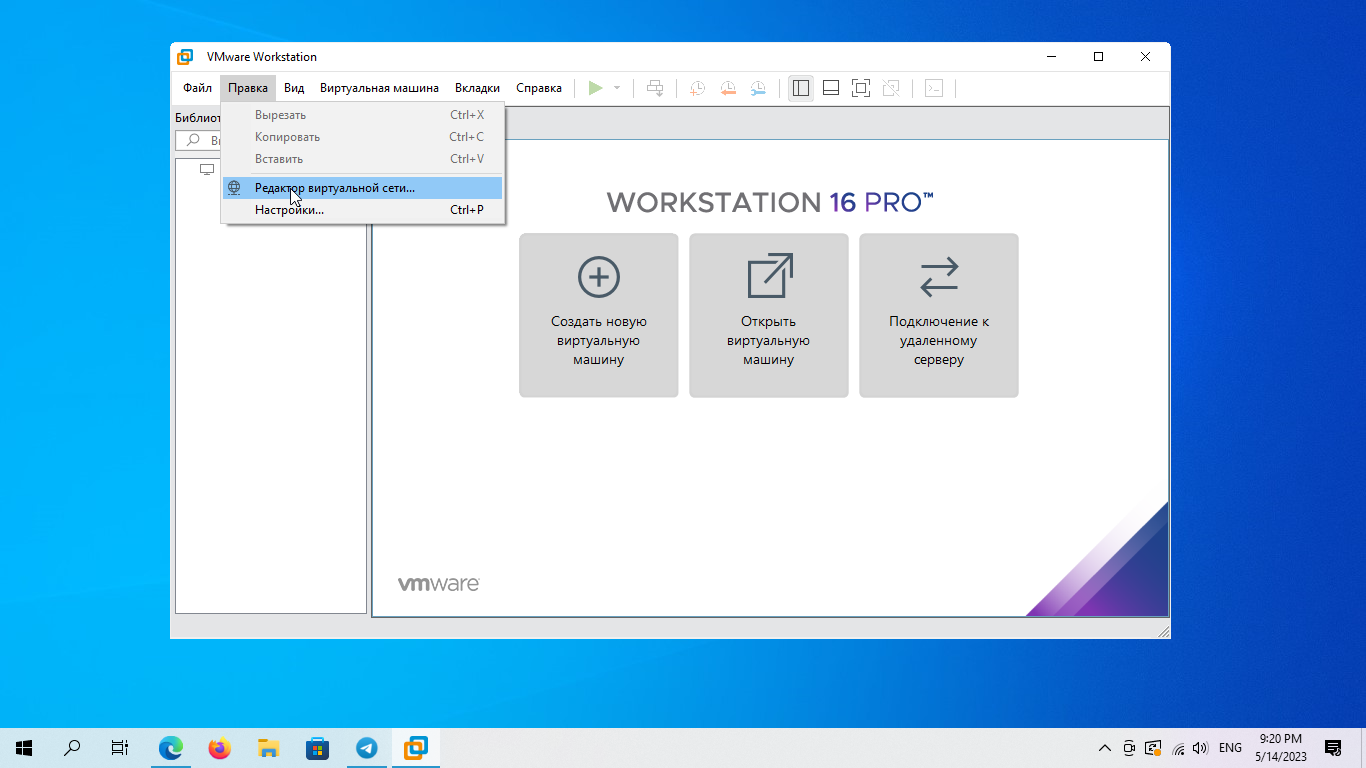
\includegraphics[width=0.85\textwidth]{5_0002}
    \label{img:2}
    \caption{Открываем редактор виртуальной сети}
  \end{figure}

  \begin{figure}[H]
    \centering
    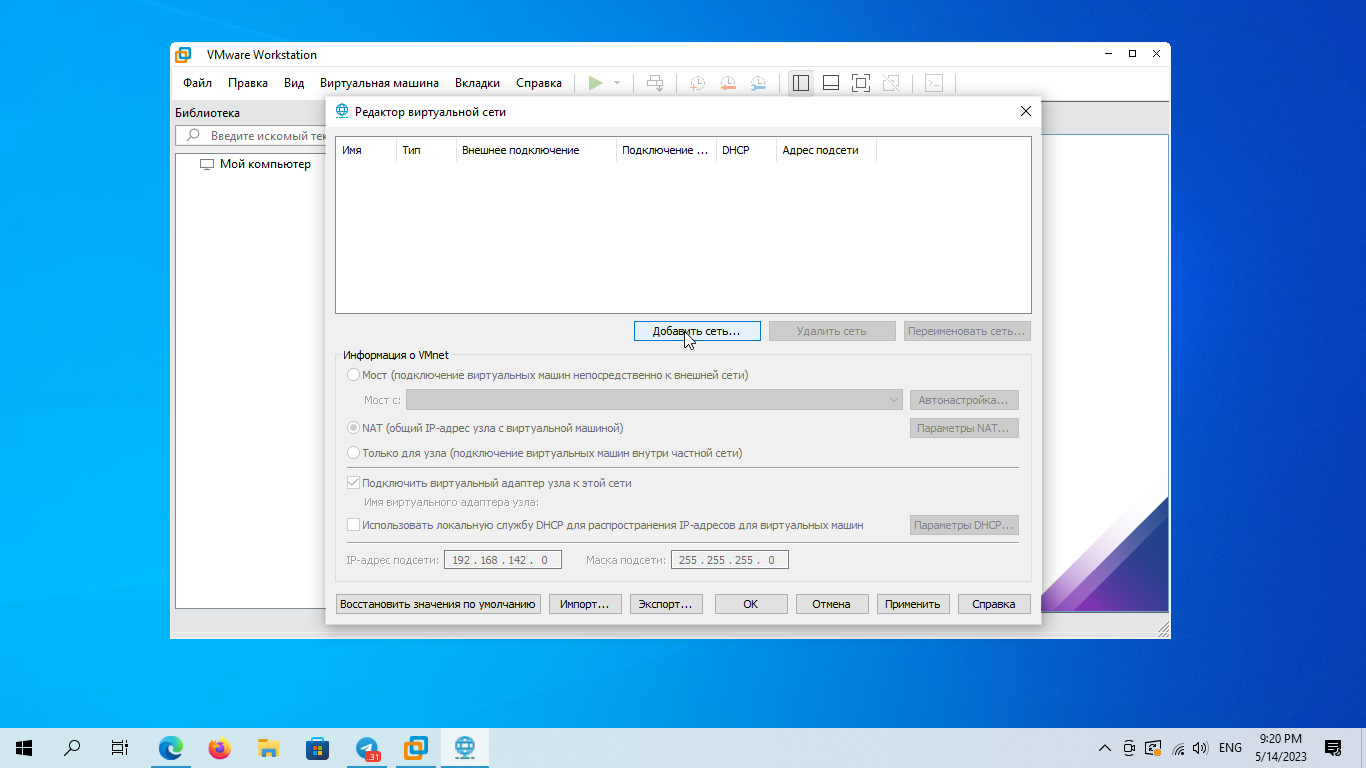
\includegraphics[width=0.85\textwidth]{5_0003}
    \label{img:3}
    \caption{Добавляем новую сеть}
  \end{figure}

  \begin{figure}[H]
    \centering
    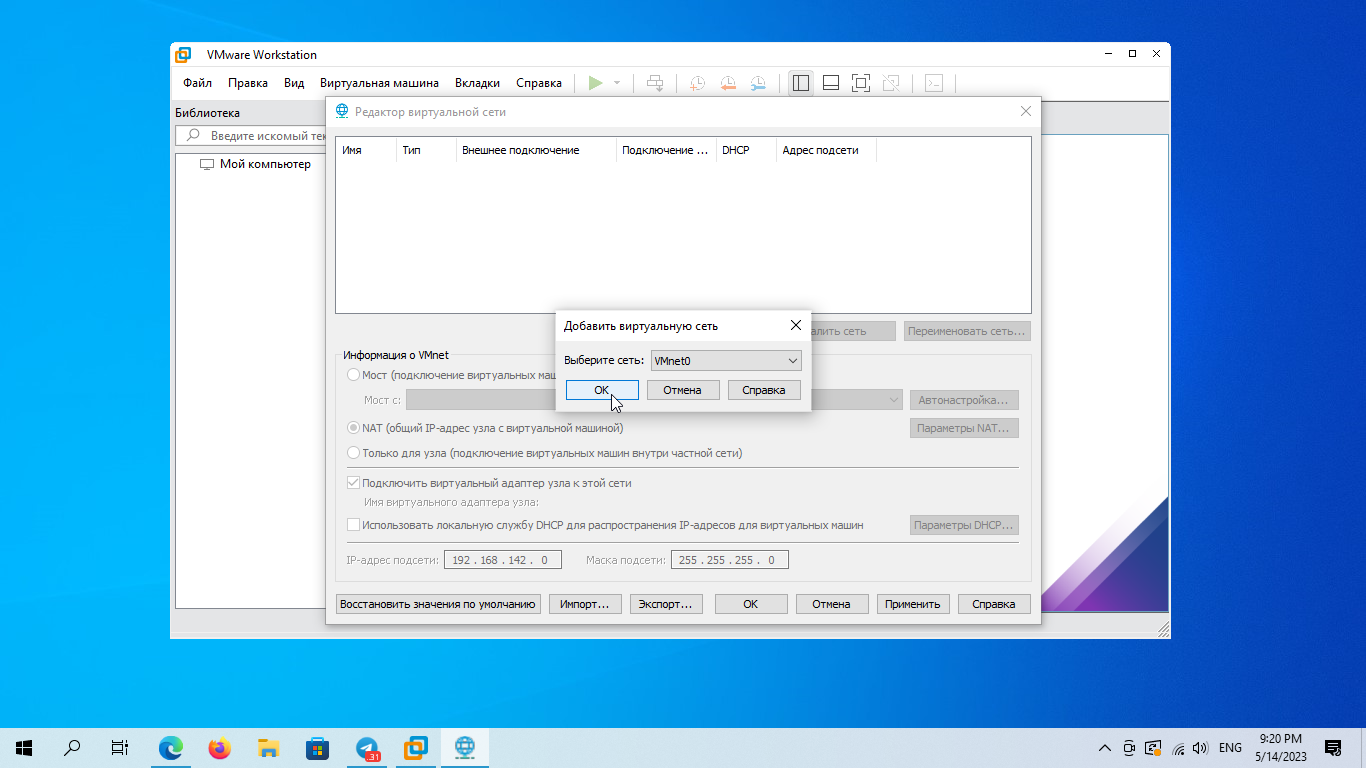
\includegraphics[width=0.85\textwidth]{5_0004}
    \label{img:4}
    \caption{Указываем ее имя}
  \end{figure}

  \begin{figure}[H]
    \centering
    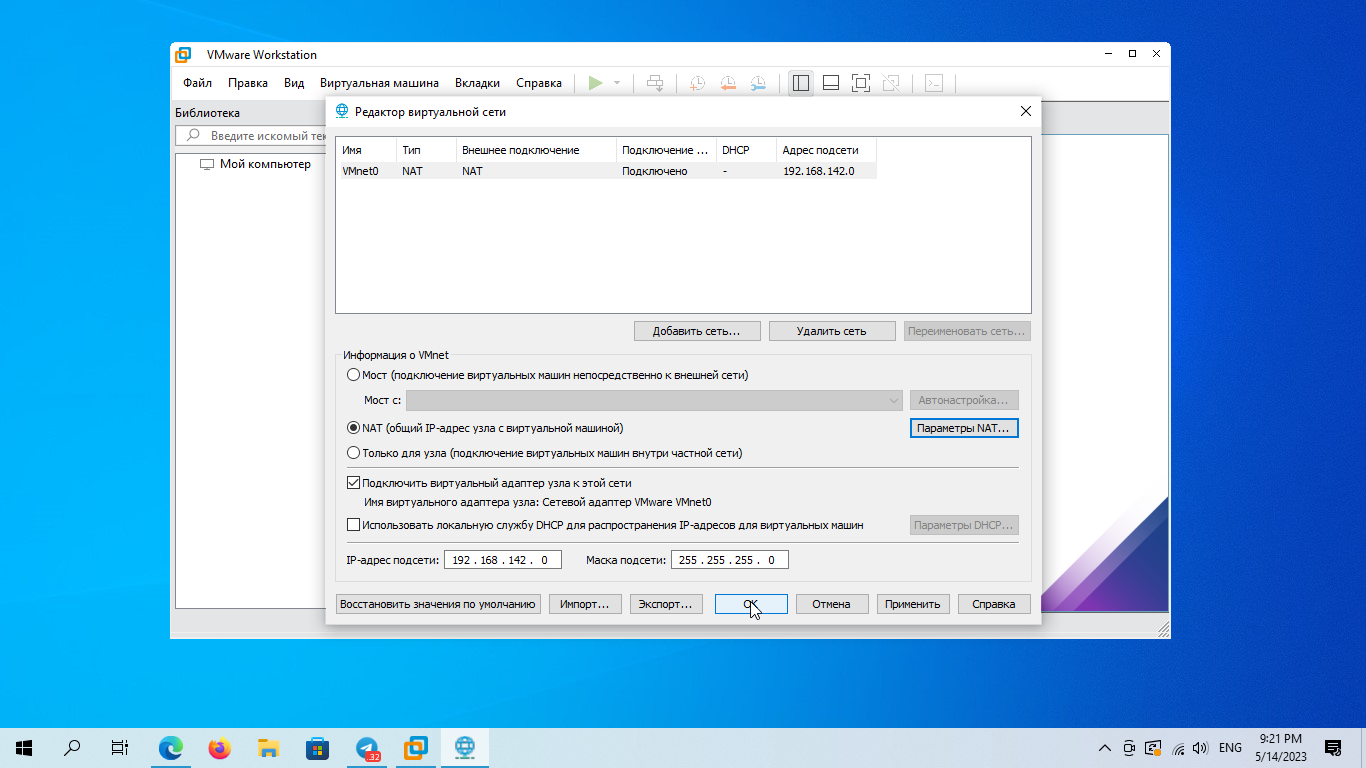
\includegraphics[width=0.85\textwidth]{5_0005}
    \label{img:5}
    \caption{Вводим Основные параметры}
  \end{figure}

  Данная сеть имеет адрес 192.168.142.0/24 с адресом шлюза 192.168.142.1 (его
  же можно использовать как адрес \textit{DNS} серера):

  \begin{figure}[H]
    \centering
    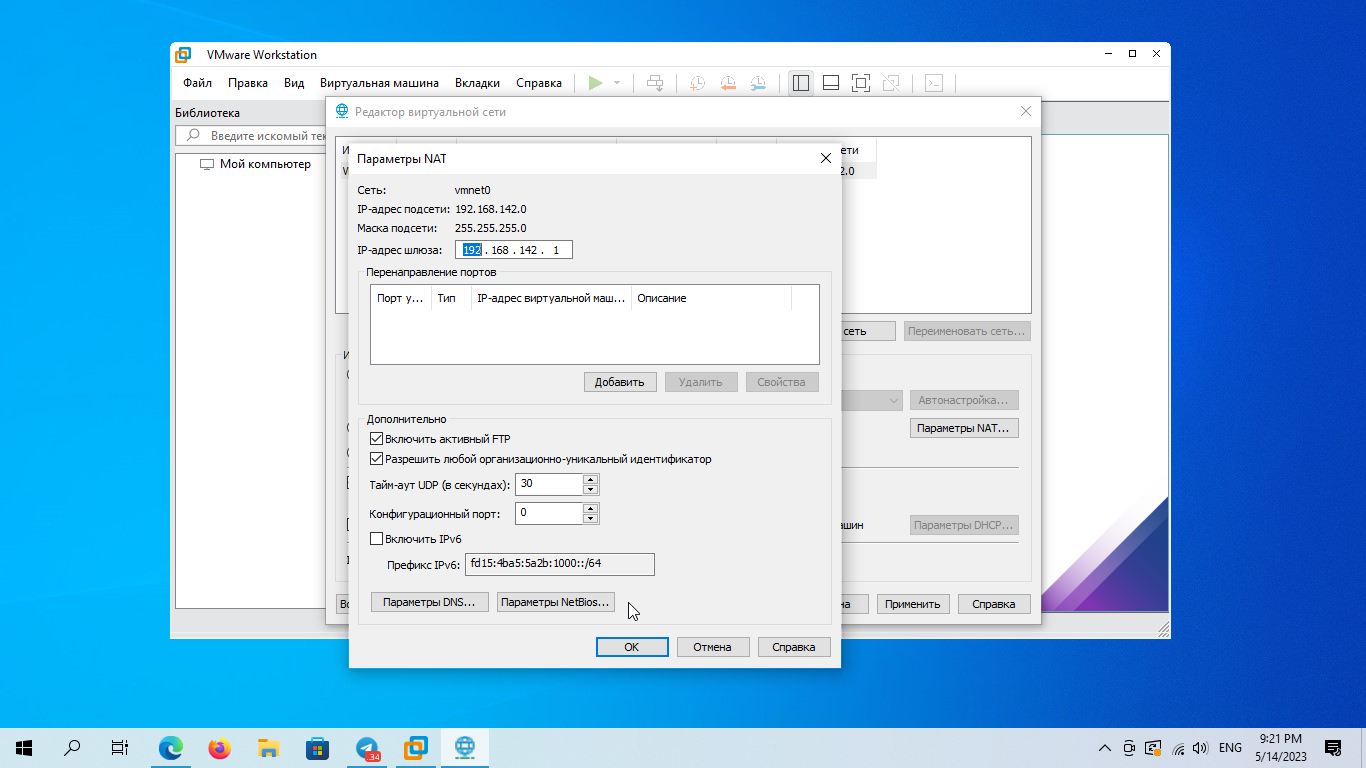
\includegraphics[width=0.85\textwidth]{5_0006}
    \label{img:6}
    \caption{Настройка шлюза}
  \end{figure}

  \subsection{Настройка серверной машины}

  Будем использовать заранее подготовленный образ с Windows Server:

  \begin{figure}[H]
    \centering
    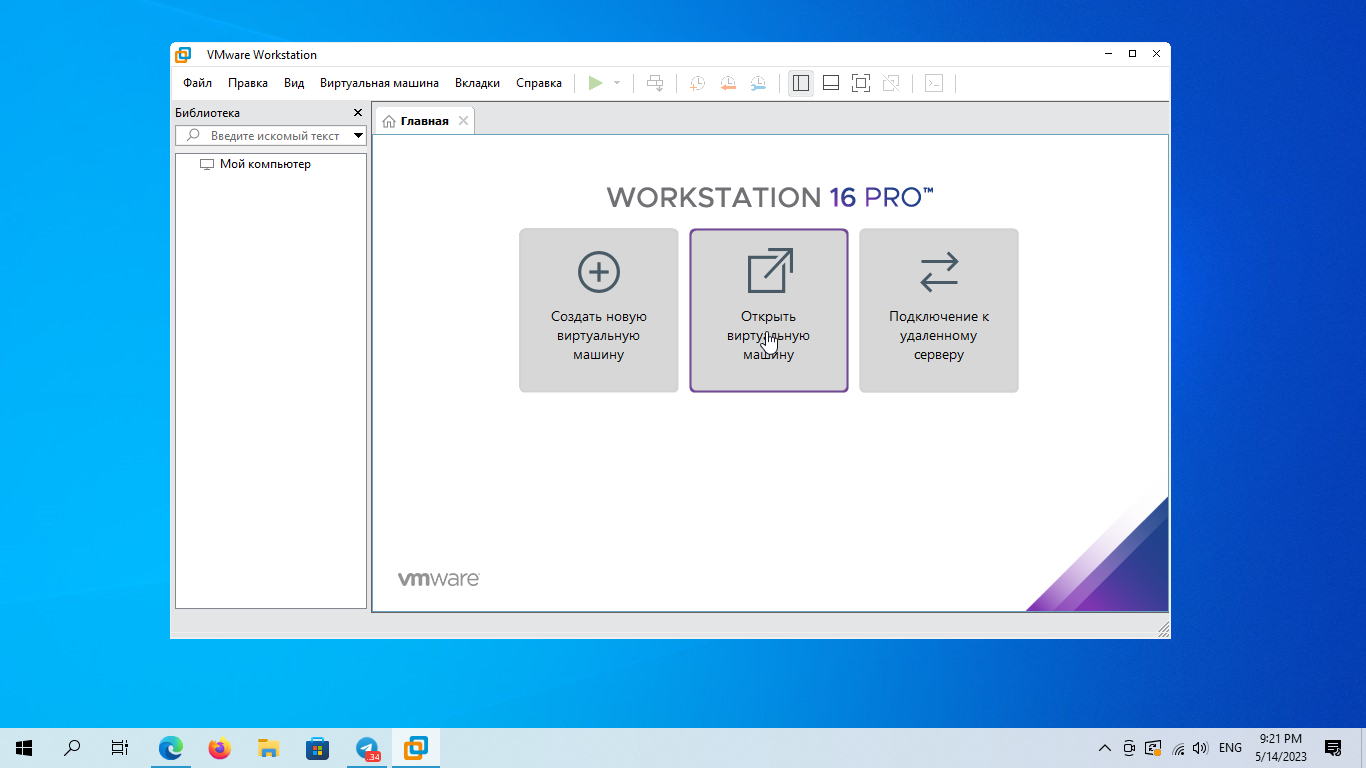
\includegraphics[width=0.85\textwidth]{5_0007}
    \label{img:7}
    \caption{Начинаем импорт ВМ}
  \end{figure}

  \begin{figure}[H]
    \centering
    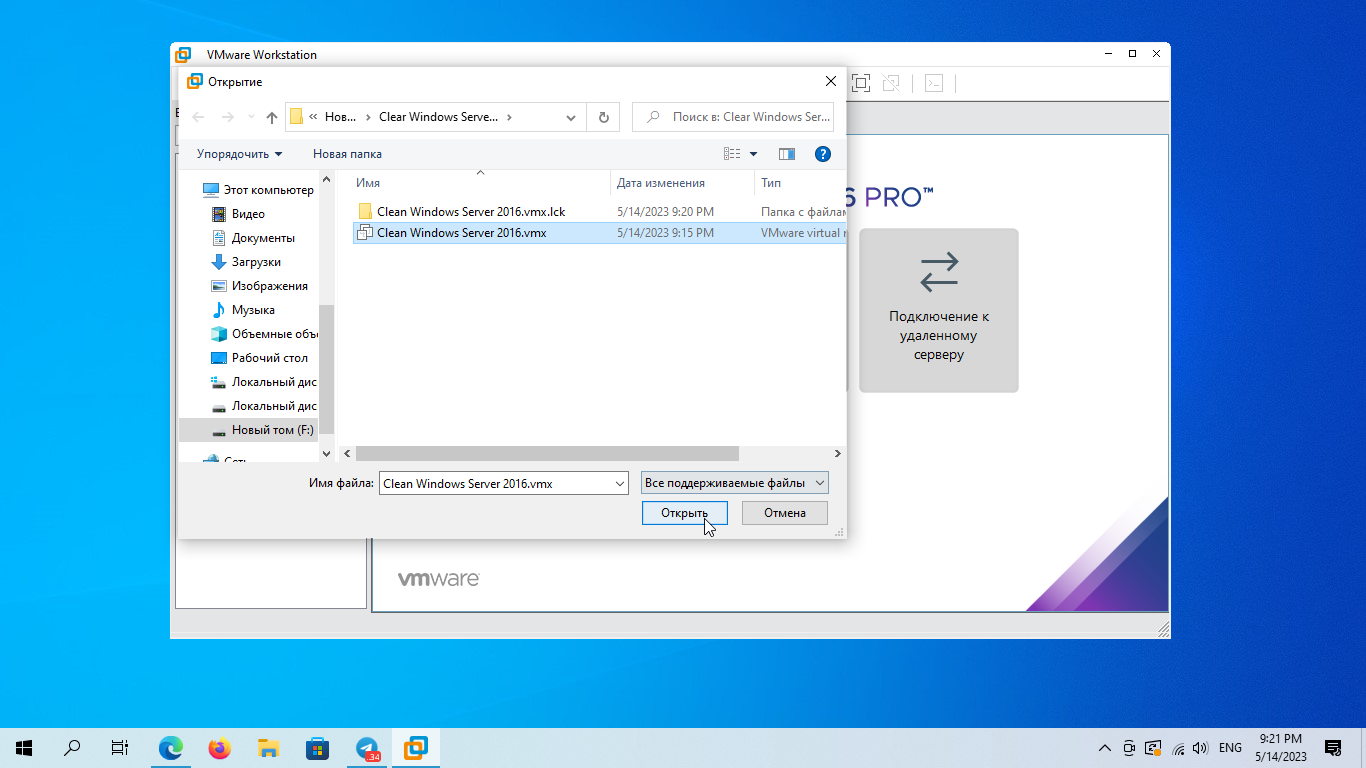
\includegraphics[width=0.85\textwidth]{5_0008}
    \label{img:8}
    \caption{Указываем путь до образа}
  \end{figure}

  \begin{figure}[H]
    \centering
    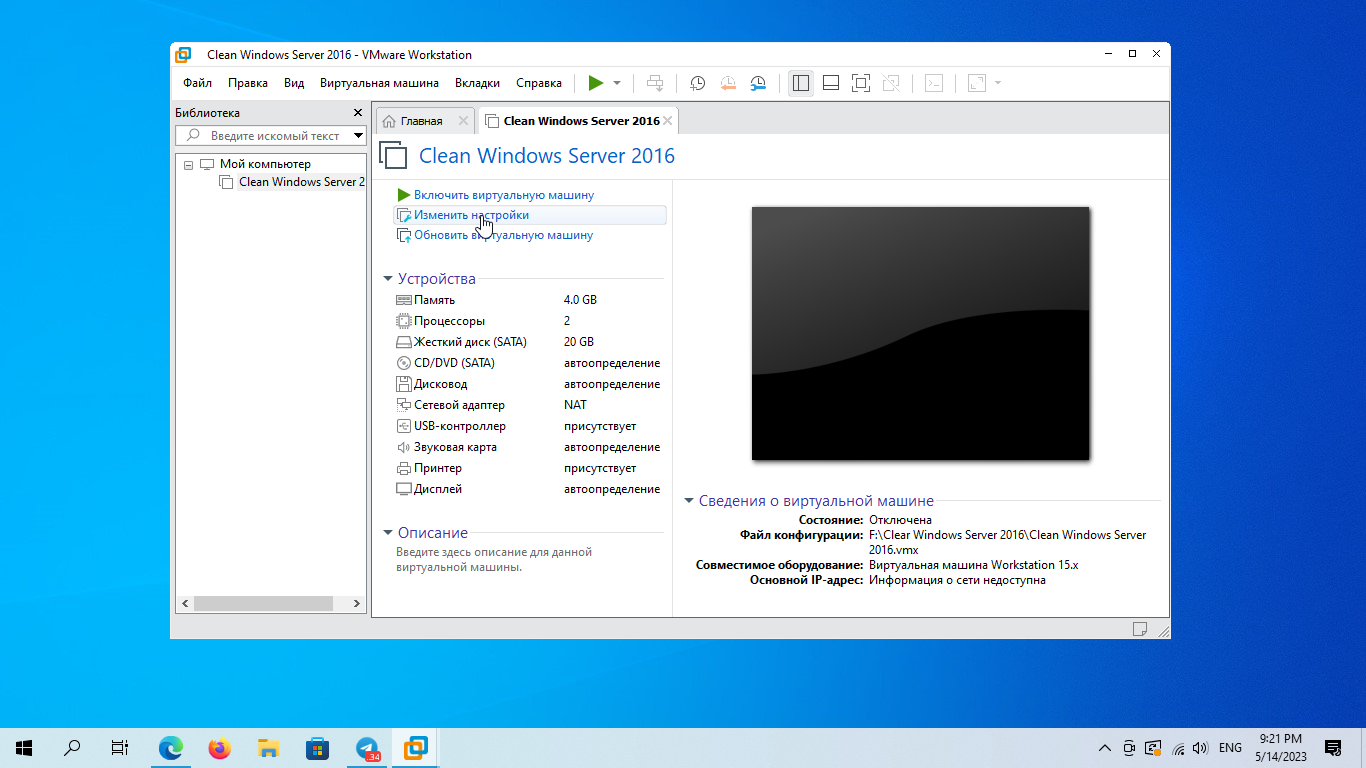
\includegraphics[width=0.85\textwidth]{5_0009}
    \label{img:9}
    \caption{Переходим к настройкам ВМ}
  \end{figure}

  \begin{figure}[H]
    \centering
    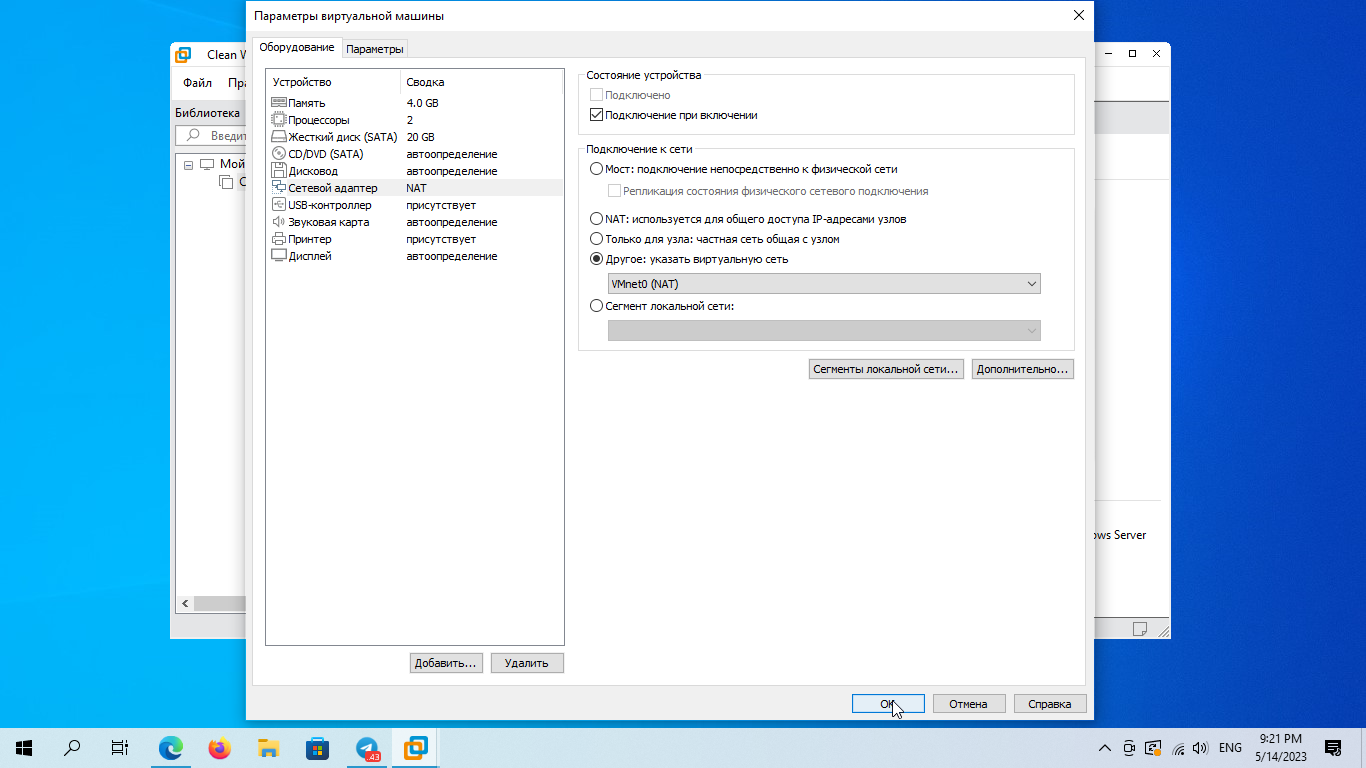
\includegraphics[width=0.85\textwidth]{5_0010}
    \label{img:10}
    \caption{Подключаем сетевой адаптер к нужной сети}
  \end{figure}

  \subsubsection{Задание IP адреса}
  
  \begin{figure}[H]
    \centering
    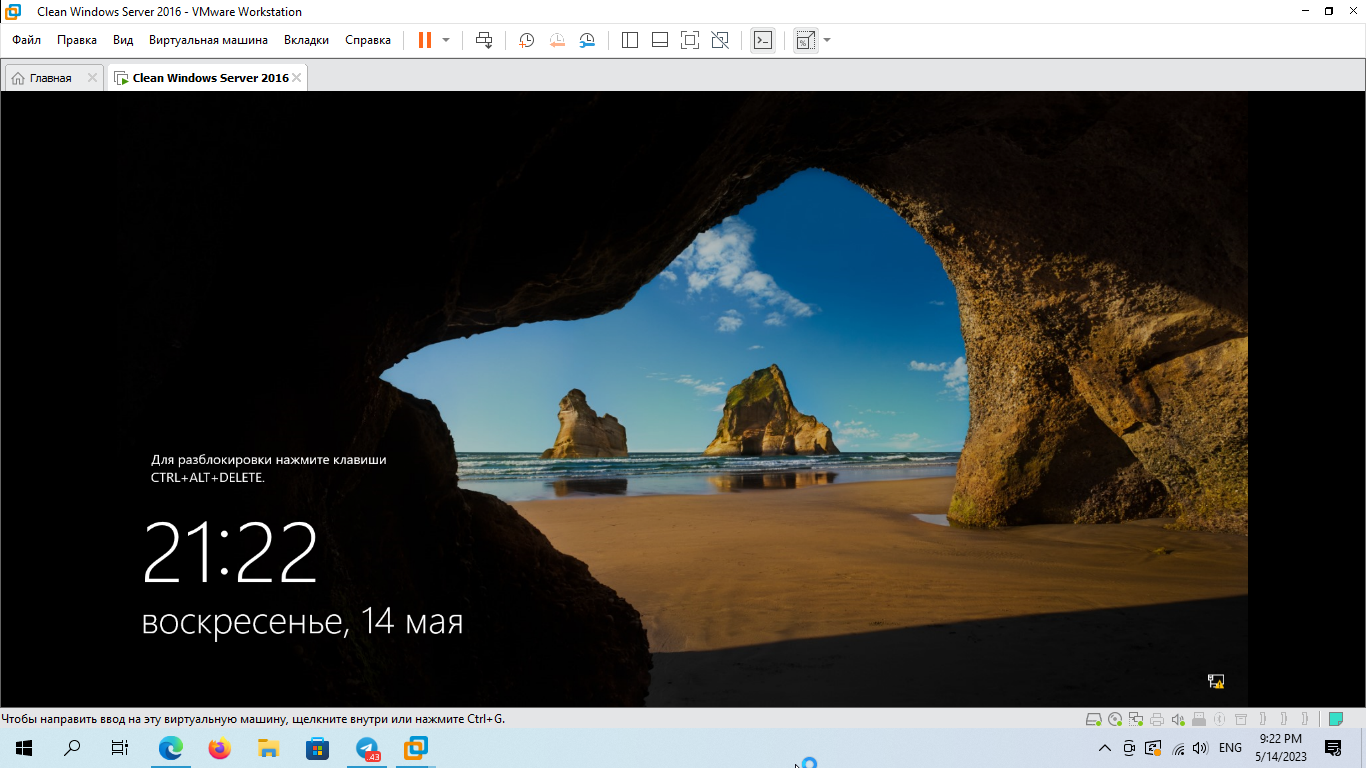
\includegraphics[width=0.85\textwidth]{5_0011}
    \label{img:11}
    \caption{Запускаем машину}
  \end{figure}

  \begin{figure}[H]
    \centering
    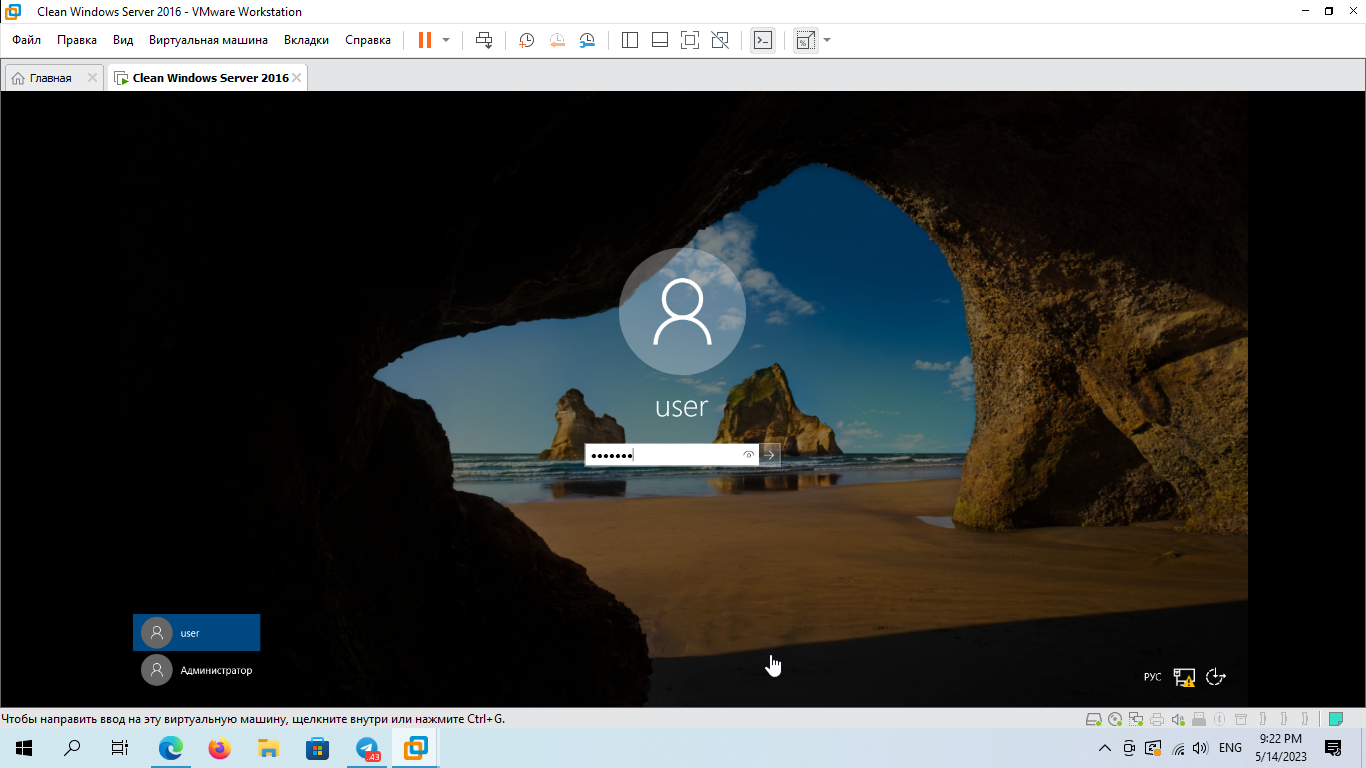
\includegraphics[width=0.85\textwidth]{5_0012}
    \label{img:12}
    \caption{Входим в учетную запиьс пользователя}
  \end{figure}

  \begin{figure}[H]
    \centering
    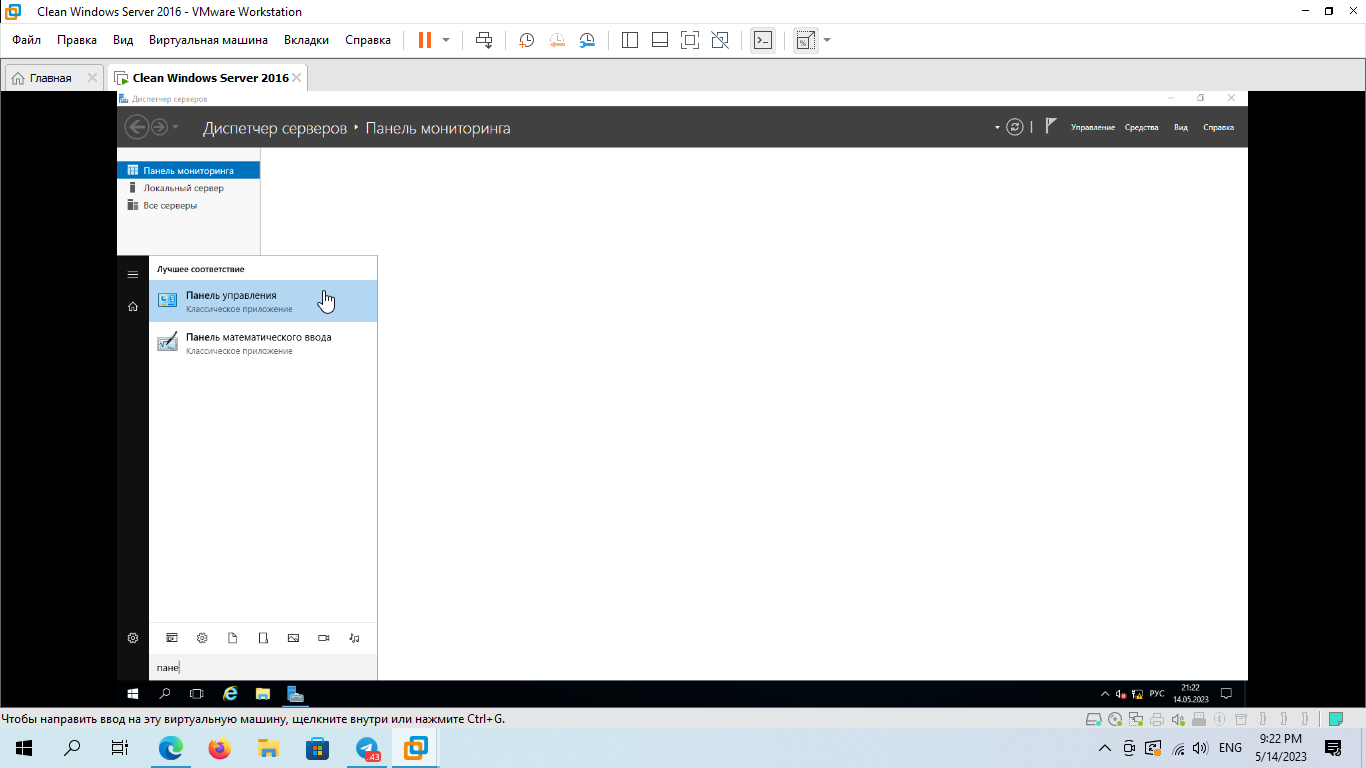
\includegraphics[width=0.85\textwidth]{5_0013}
    \label{img:13}
    \caption{Открываем панель задач}
  \end{figure}

  \begin{figure}[H]
    \centering
    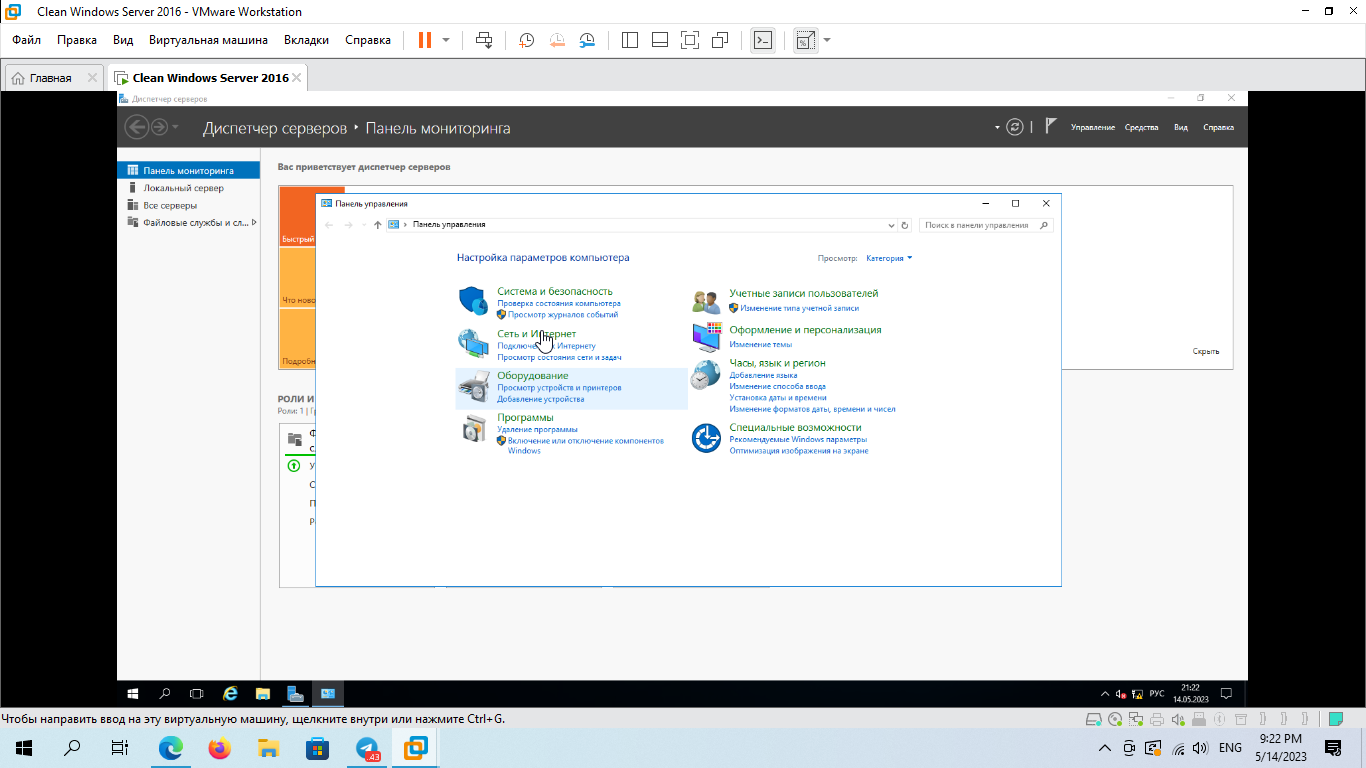
\includegraphics[width=0.85\textwidth]{5_0014}
    \label{img:14}
    \caption{Настройки сети и Интернета}
  \end{figure}

  \begin{figure}[H]
    \centering
    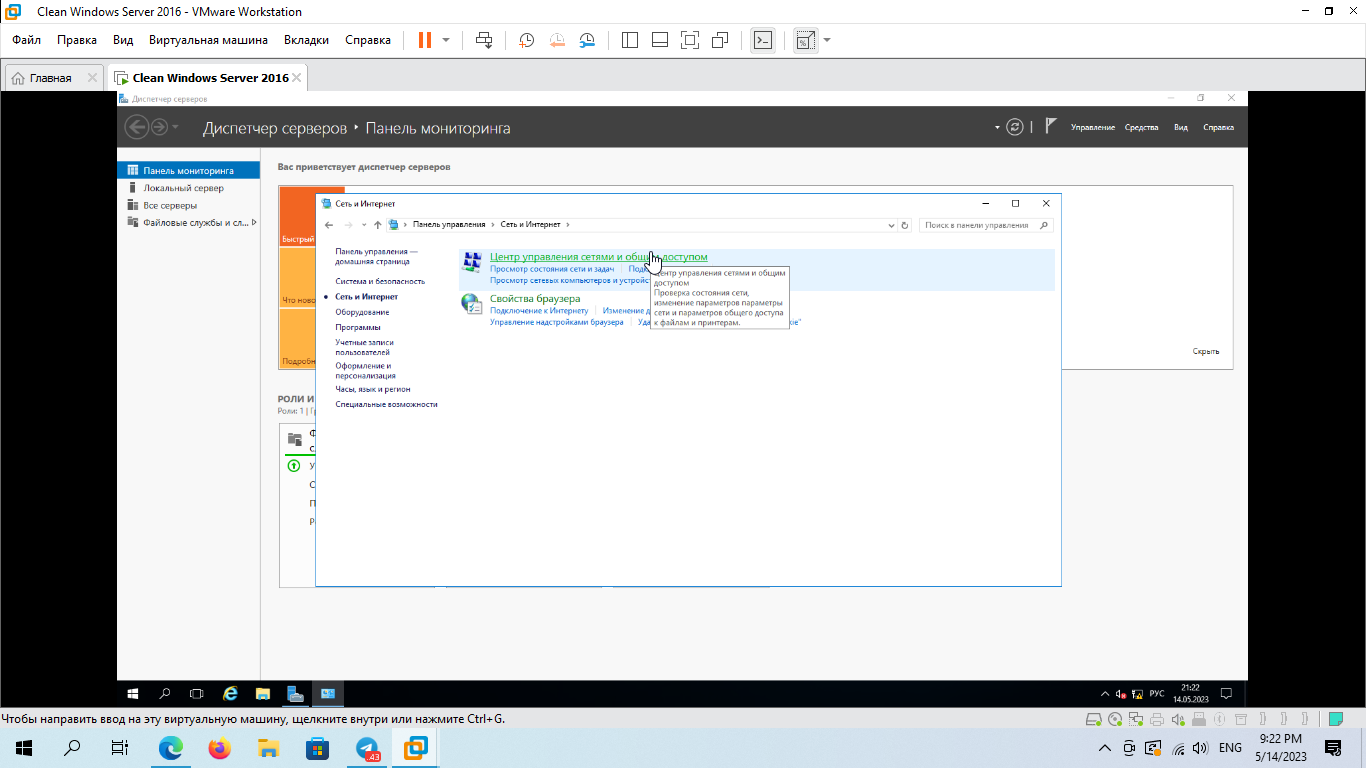
\includegraphics[width=0.85\textwidth]{5_0015}
    \label{img:15}
    \caption{Открываем центр управления сетями и общим доступом}
  \end{figure}

  \begin{figure}[H]
    \centering
    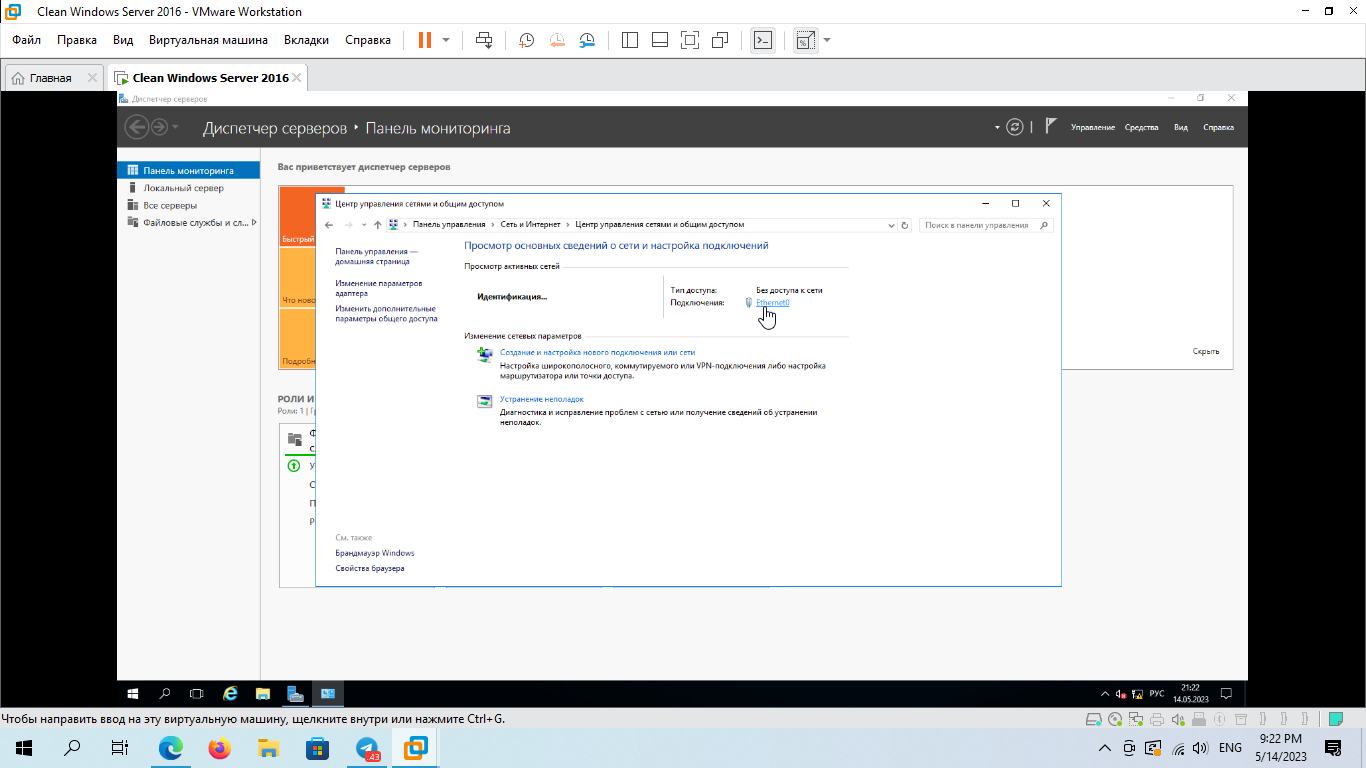
\includegraphics[width=0.85\textwidth]{5_0016}
    \label{img:16}
    \caption{Выбираем необходимый сетевой интерфейс}
  \end{figure}

  \begin{figure}[H]
    \centering
    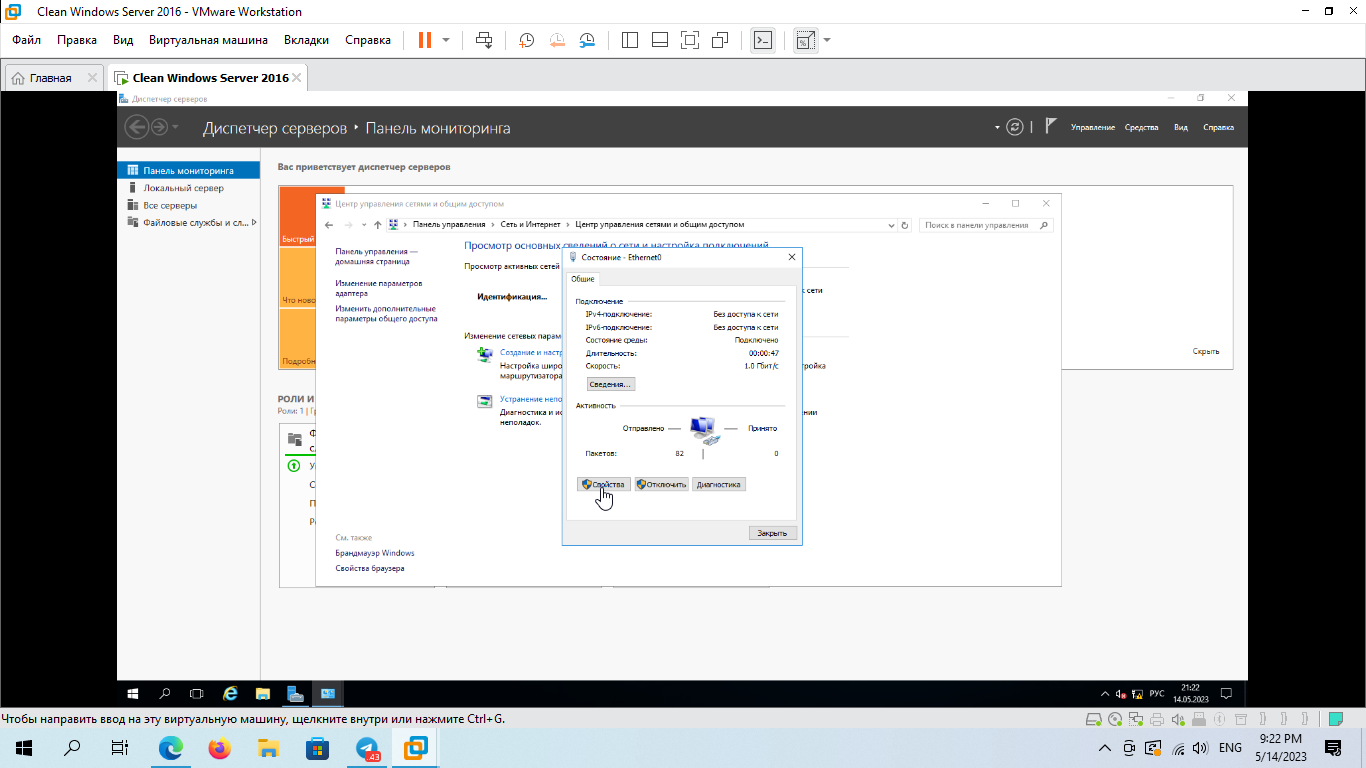
\includegraphics[width=0.85\textwidth]{5_0017}
    \label{img:17}
    \caption{Заходим в его свойства}
  \end{figure}

  \begin{figure}[H]
    \centering
    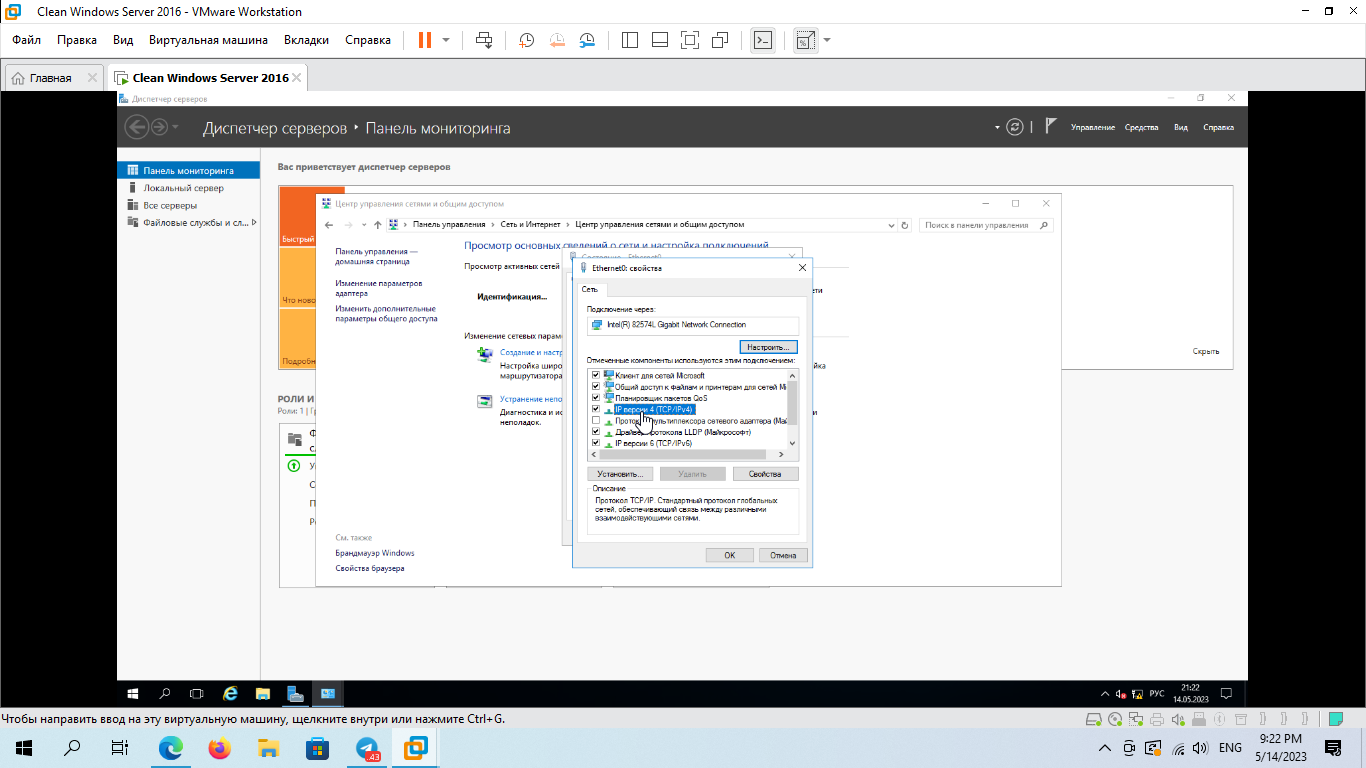
\includegraphics[width=0.85\textwidth]{5_0018}
    \label{img:18}
    \caption{Открываем параметры IPv4}
  \end{figure}

  \begin{figure}[H]
    \centering
    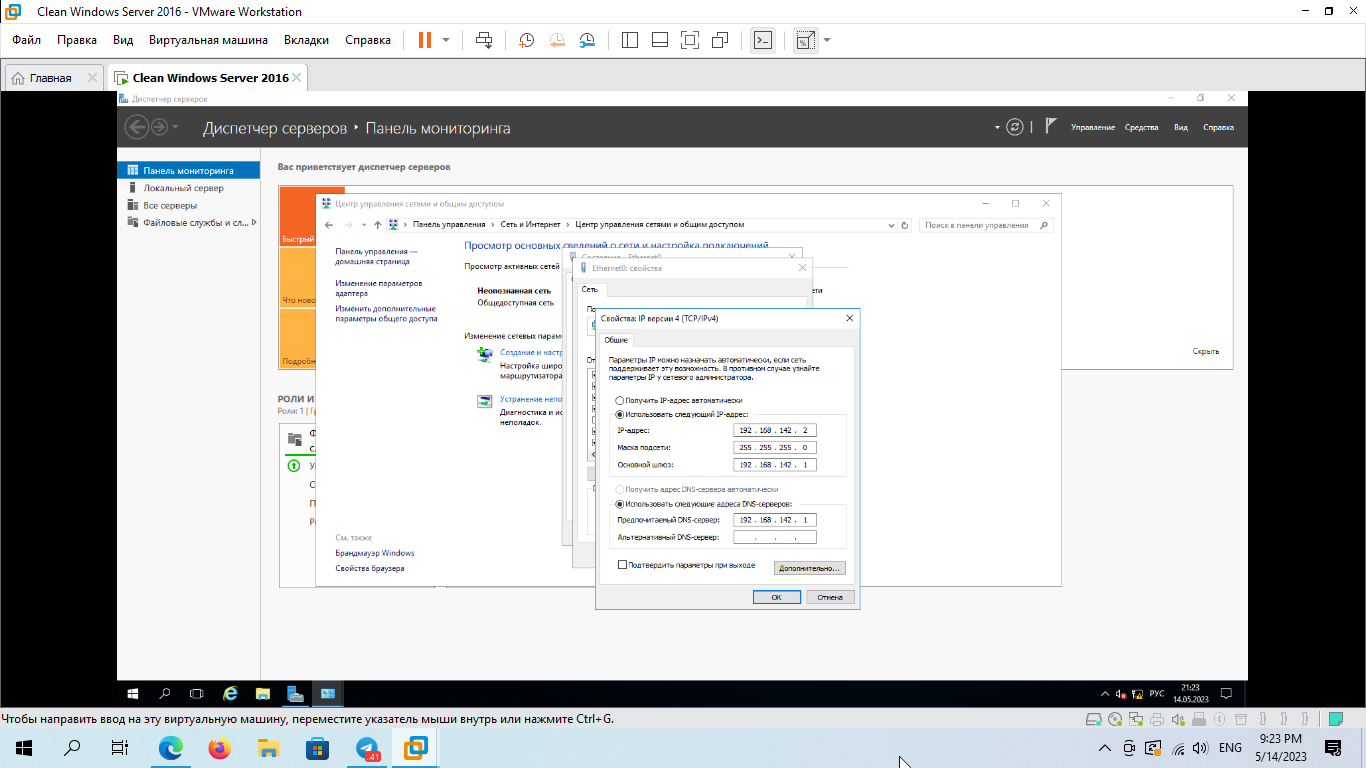
\includegraphics[width=0.85\textwidth]{5_0019}
    \label{img:19}
    \caption{Задаем IP адрес, адрес сети, маску подсети и DNS}
  \end{figure}

  Данной машине был выдан первый свободный IP адрес - 192.168.142.2.

  \begin{figure}[H]
    \centering
    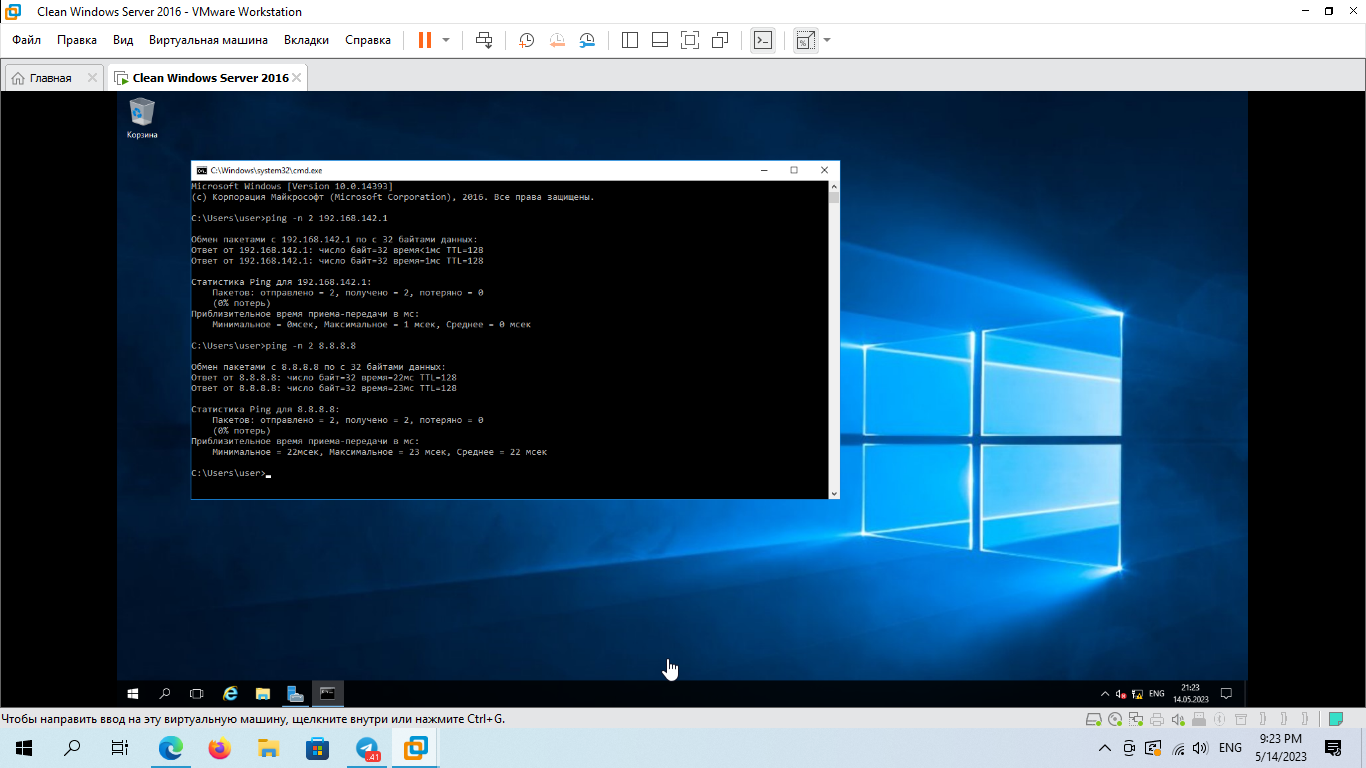
\includegraphics[width=0.85\textwidth]{5_0020}
    \label{img:20}
    \caption{Проверка доступности сети}
  \end{figure}

  \begin{figure}[H]
    \centering
    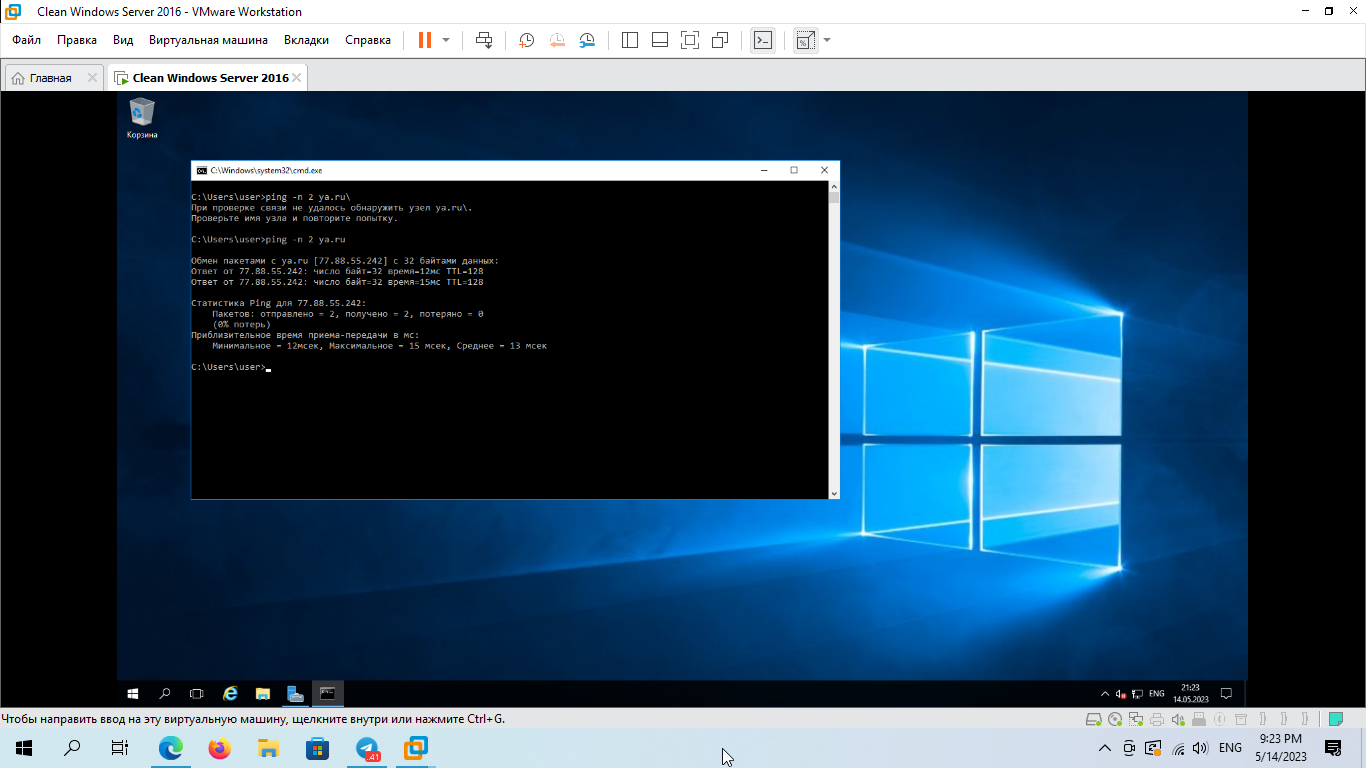
\includegraphics[width=0.85\textwidth]{5_0021}
    \label{img:21}
    \caption{Проверка работы DNS}
  \end{figure}

  \subsubsection{Настройка пароля учетной записи администратора}

  \begin{figure}[H]
    \centering
    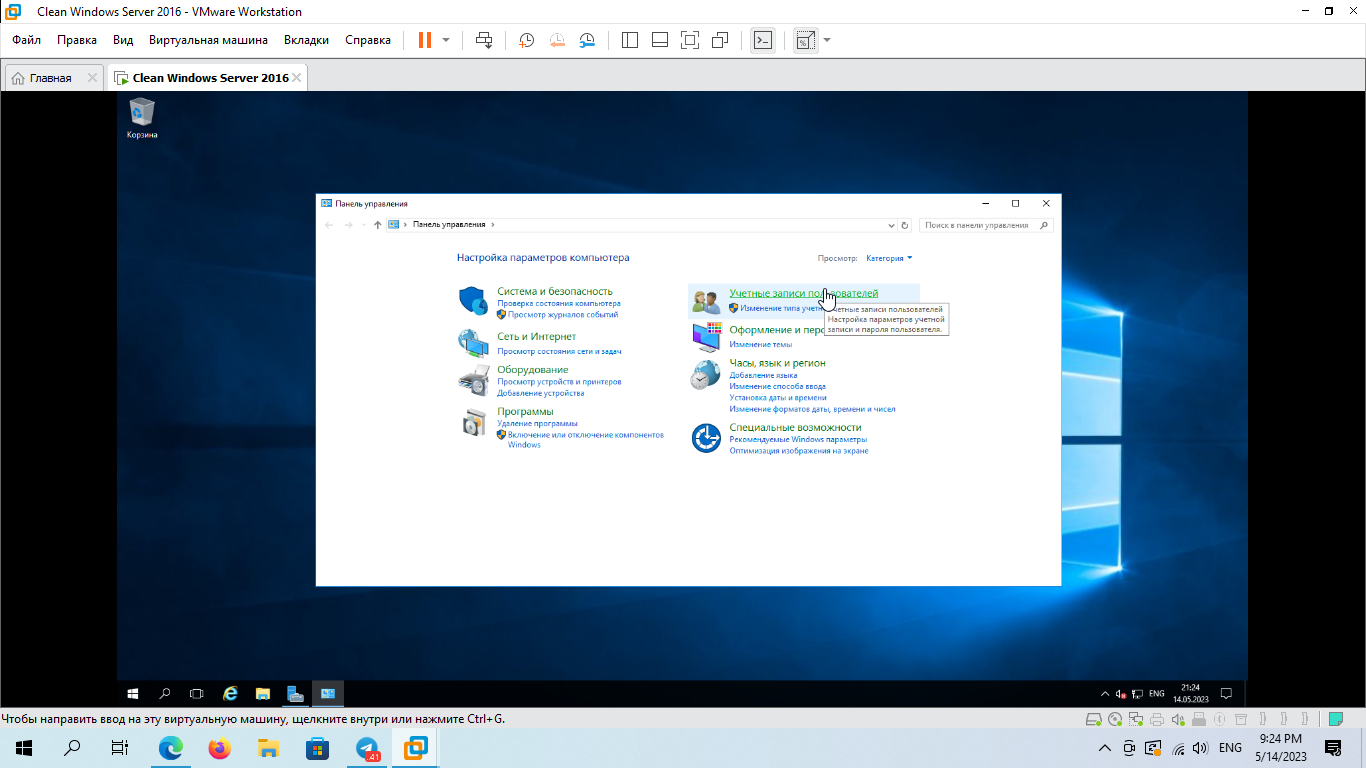
\includegraphics[width=0.85\textwidth]{5_0022}
    \label{img:22}
    \caption{Переходим в учетные записи пользователей}
  \end{figure}

  \begin{figure}[H]
    \centering
    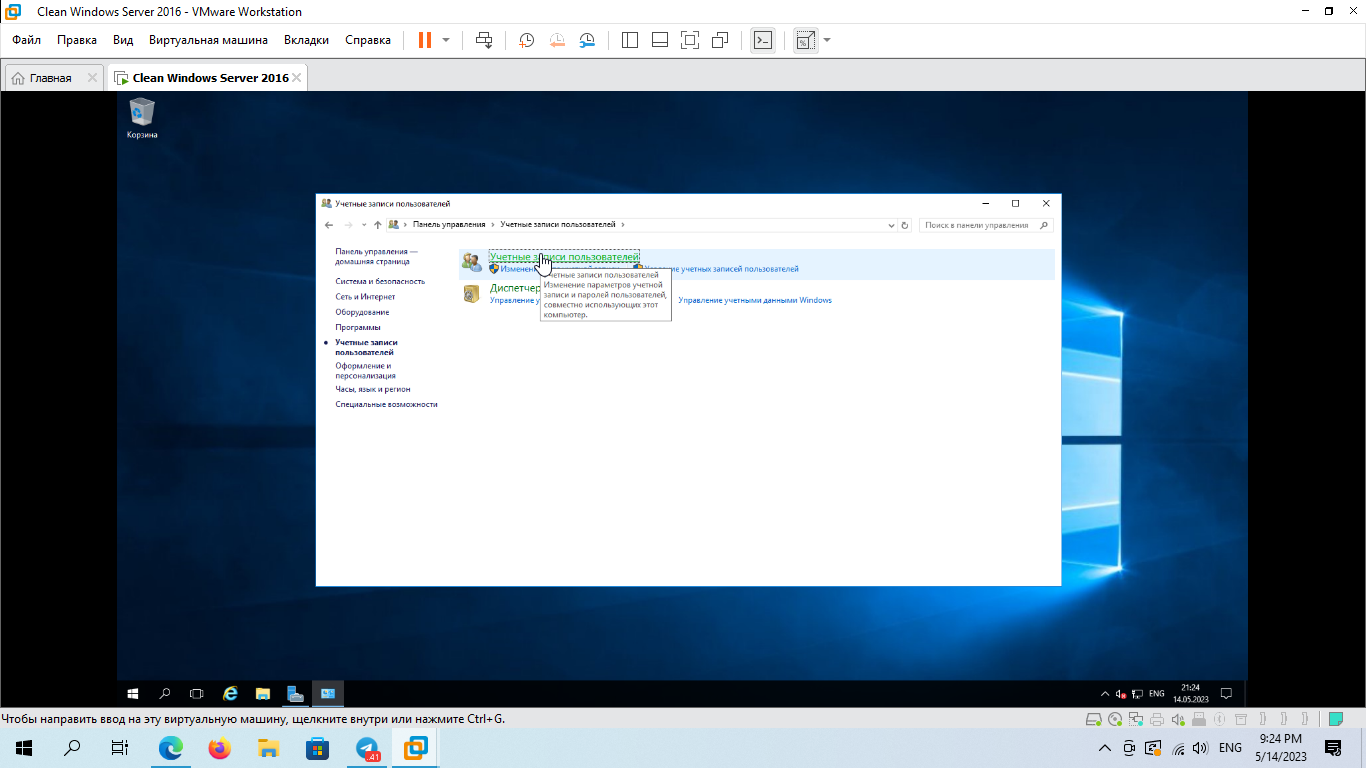
\includegraphics[width=0.85\textwidth]{5_0023}
    \label{img:23}
    \caption{Учетные записи пользователей}
  \end{figure}

  \begin{figure}[H]
    \centering
    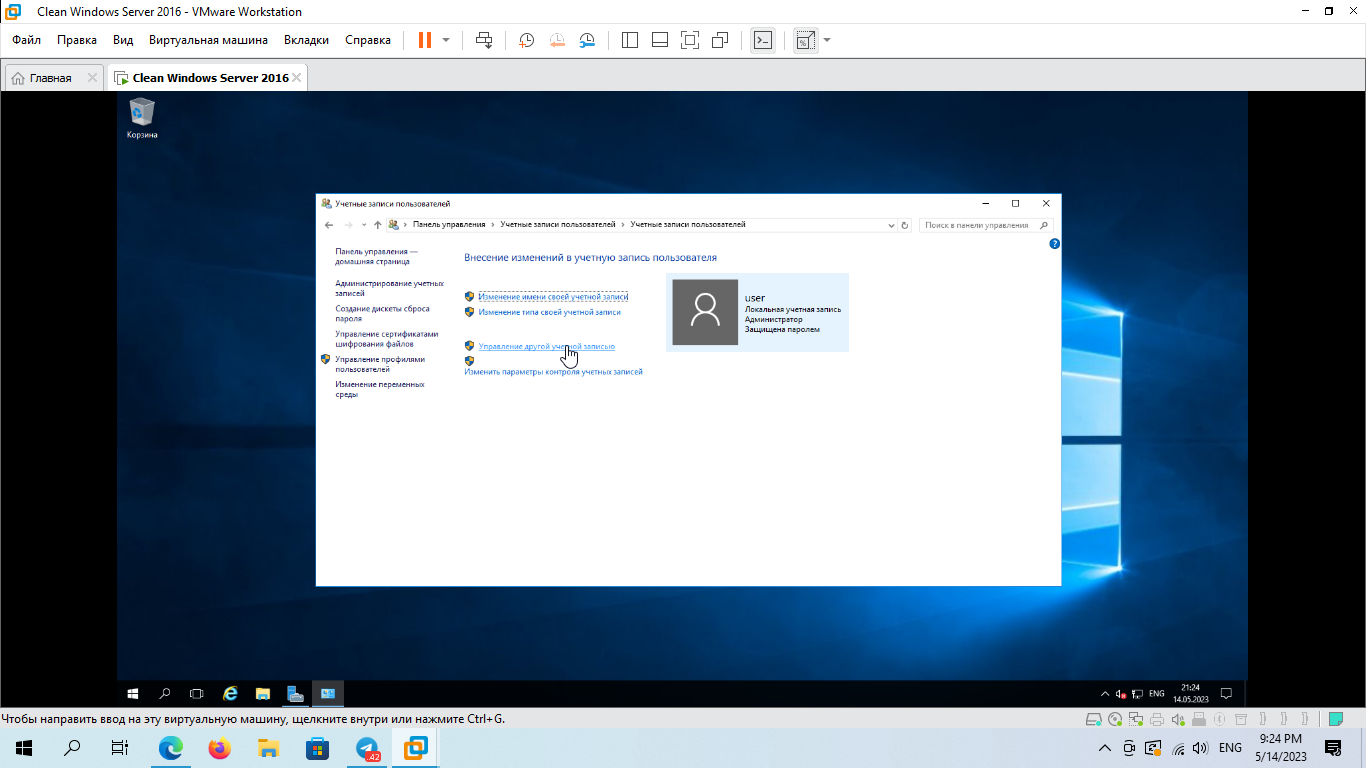
\includegraphics[width=0.85\textwidth]{5_0024}
    \label{img:24}
    \caption{Переходим к управлению другой учетной записью}
  \end{figure}

  \begin{figure}[H]
    \centering
    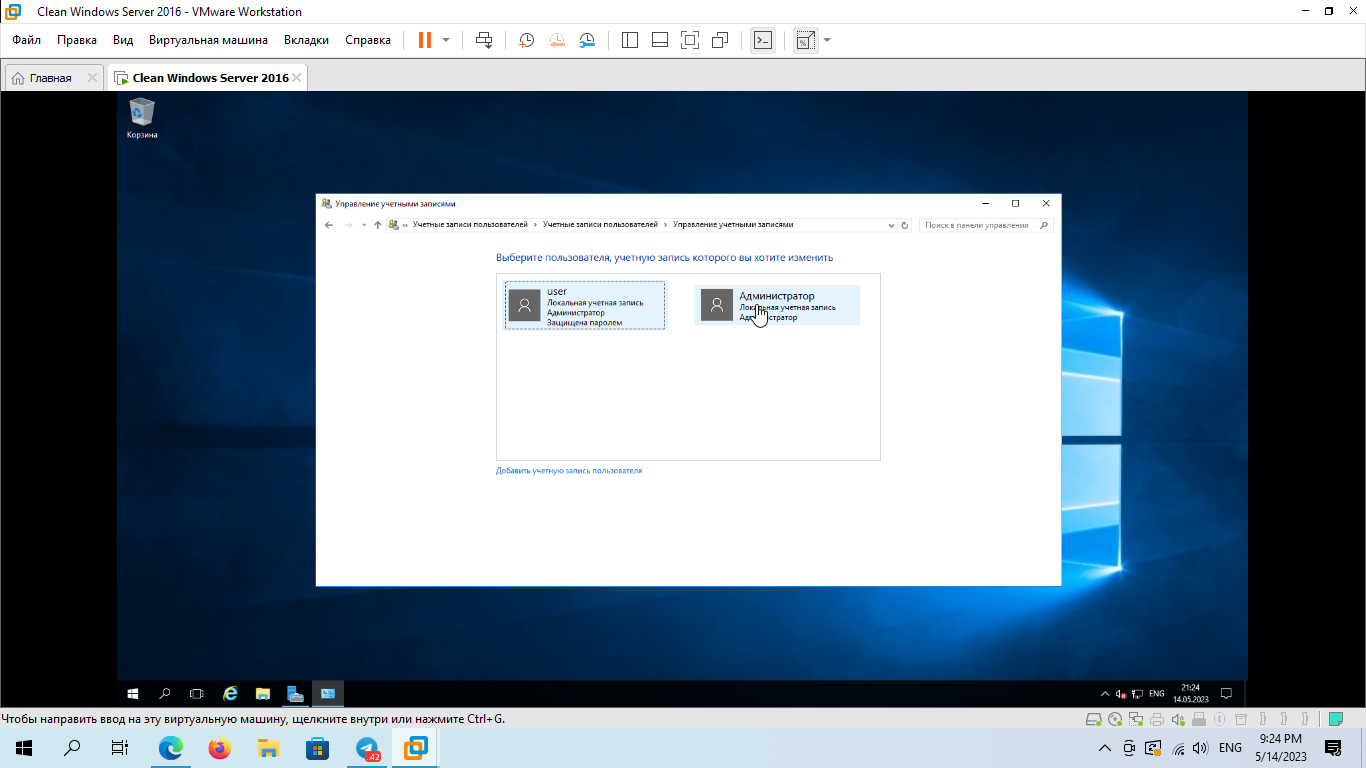
\includegraphics[width=0.85\textwidth]{5_0025}
    \label{img:25}
    \caption{Выбираем запись администратора}
  \end{figure}

  \begin{figure}[H]
    \centering
    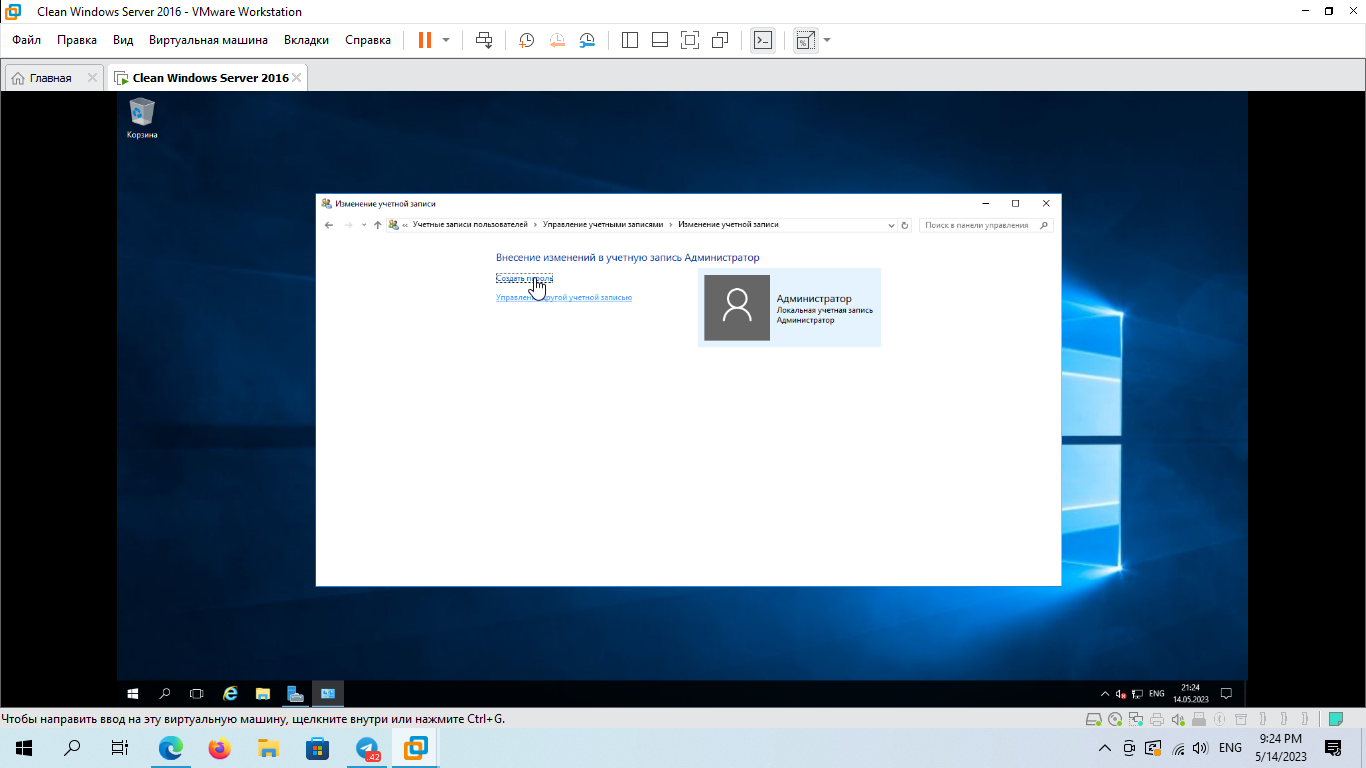
\includegraphics[width=0.85\textwidth]{5_0026}
    \label{img:26}
    \caption{Выбираем опцию создания пароля}
  \end{figure}

  \begin{figure}[H]
    \centering
    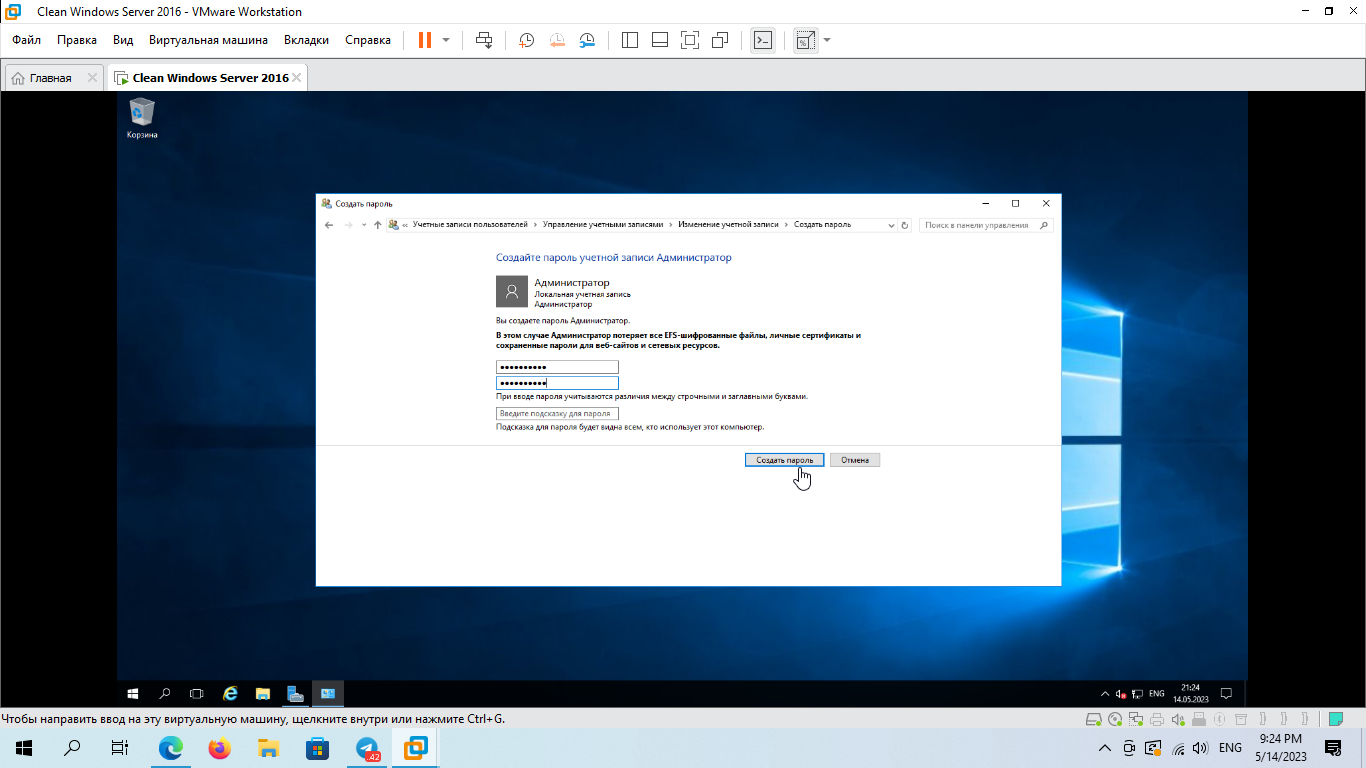
\includegraphics[width=0.85\textwidth]{5_0027}
    \label{img:27}
    \caption{Указываем пароль}
  \end{figure}

  \subsection{Создание и настройка домена}

  \subsubsection{Установка ролей и компонентов}

  Открываем диспетчер серверов и начинаем настройку:

  \begin{figure}[H]
    \centering
    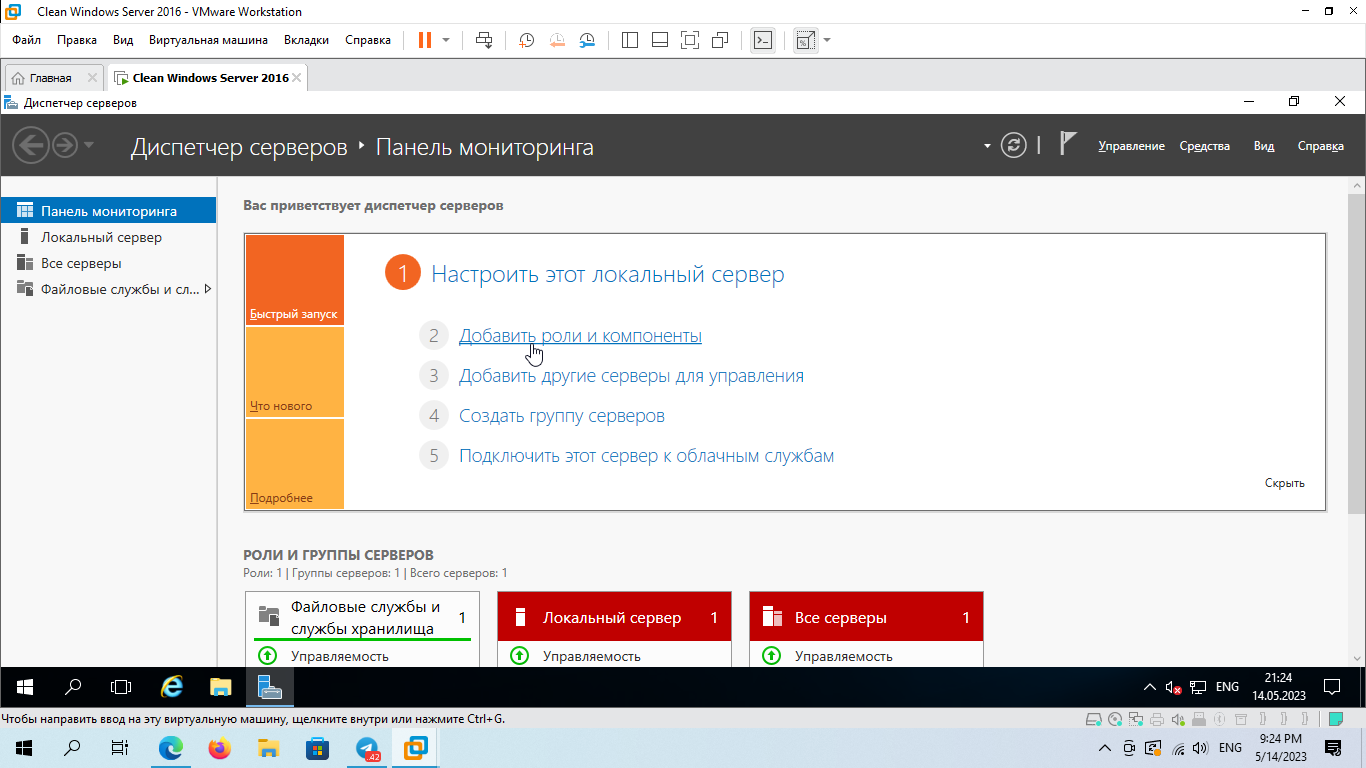
\includegraphics[width=0.85\textwidth]{5_0028}
    \label{img:28}
    \caption{Добавляем роли и компоненты}
  \end{figure}

  \begin{figure}[H]
    \centering
    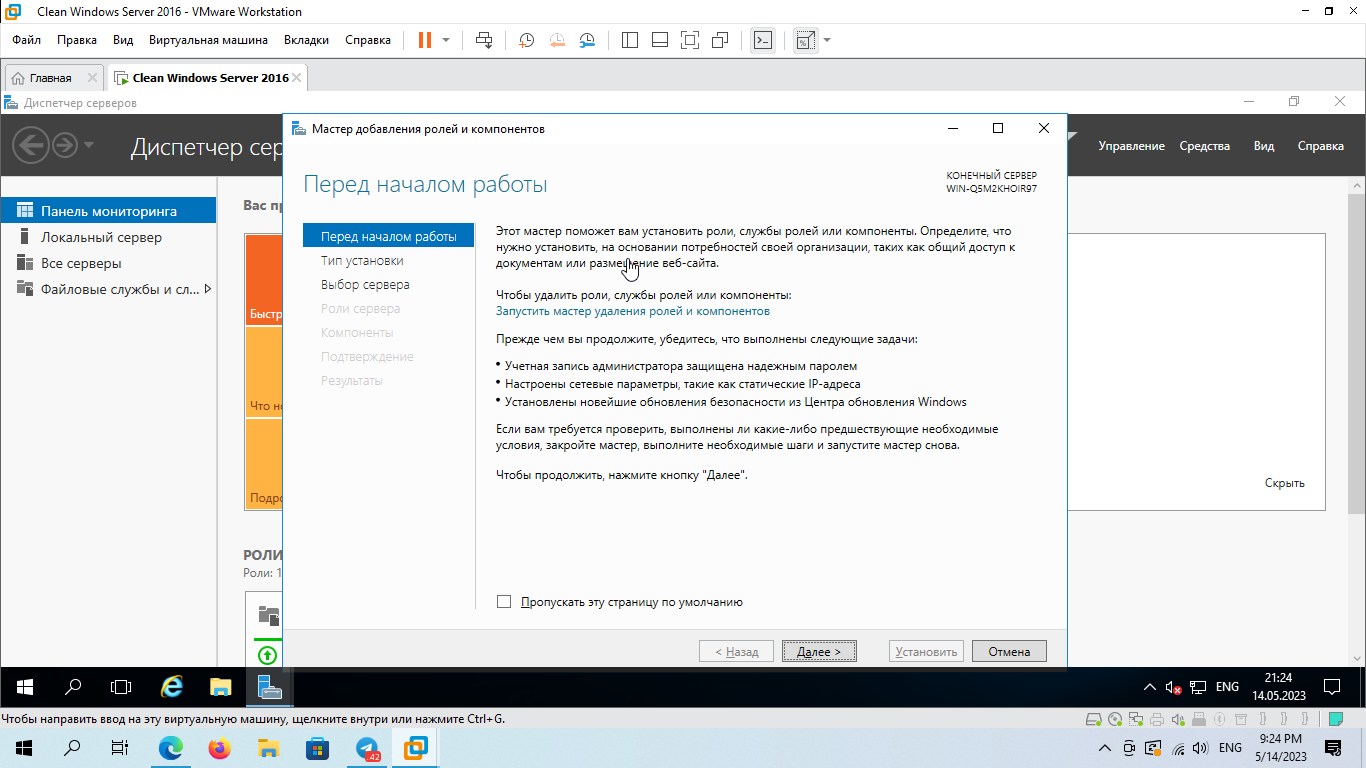
\includegraphics[width=0.85\textwidth]{5_0029}
    \label{img:29}
    \caption{Далее}
  \end{figure}

  \begin{figure}[H]
    \centering
    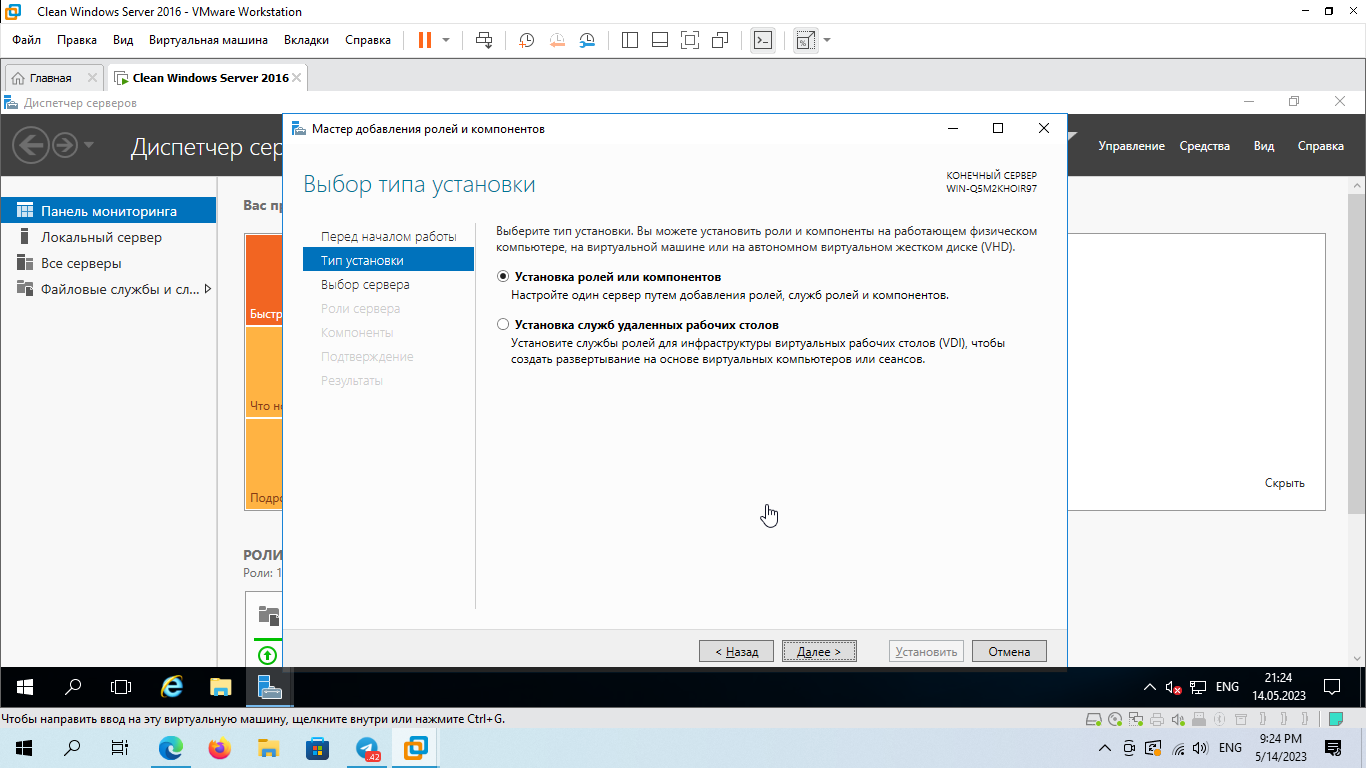
\includegraphics[width=0.85\textwidth]{5_0030}
    \label{img:30}
    \caption{Необходимы новые роли и компоненты}
  \end{figure}

  \begin{figure}[H]
    \centering
    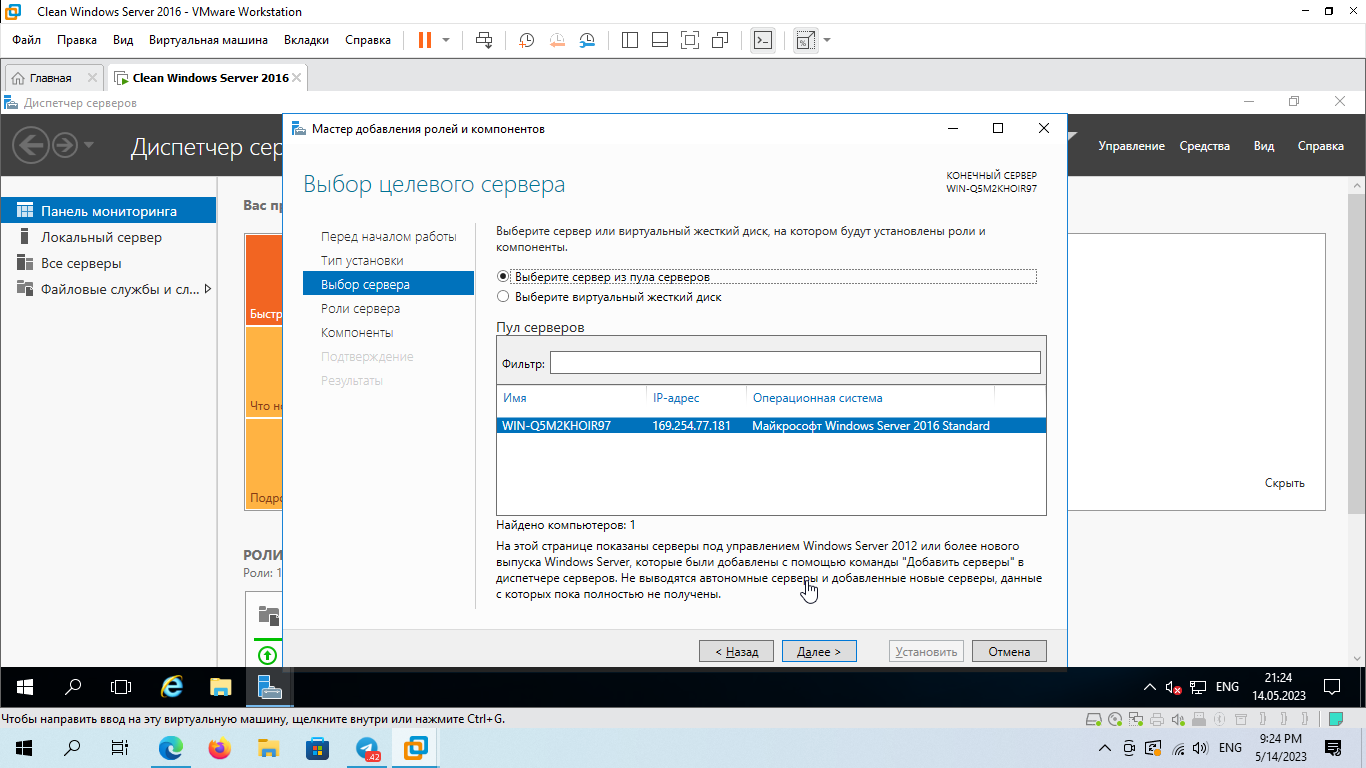
\includegraphics[width=0.85\textwidth]{5_0031}
    \label{img:31}
    \caption{Выполняем установку для текущего компьютера}
  \end{figure}

  \begin{figure}[H]
    \centering
    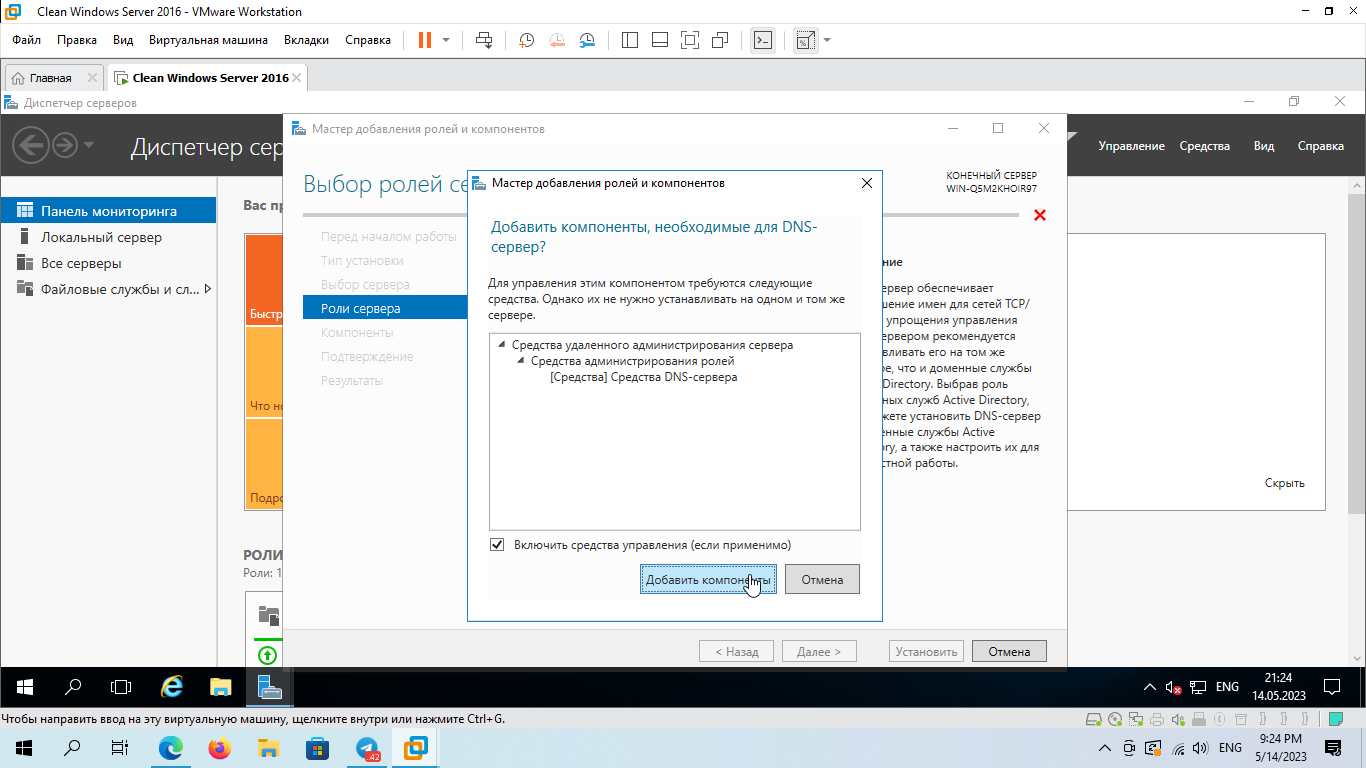
\includegraphics[width=0.85\textwidth]{5_0032}
    \label{img:32}
    \caption{Добавляем роль DNS сервера}
  \end{figure}

  \begin{figure}[H]
    \centering
    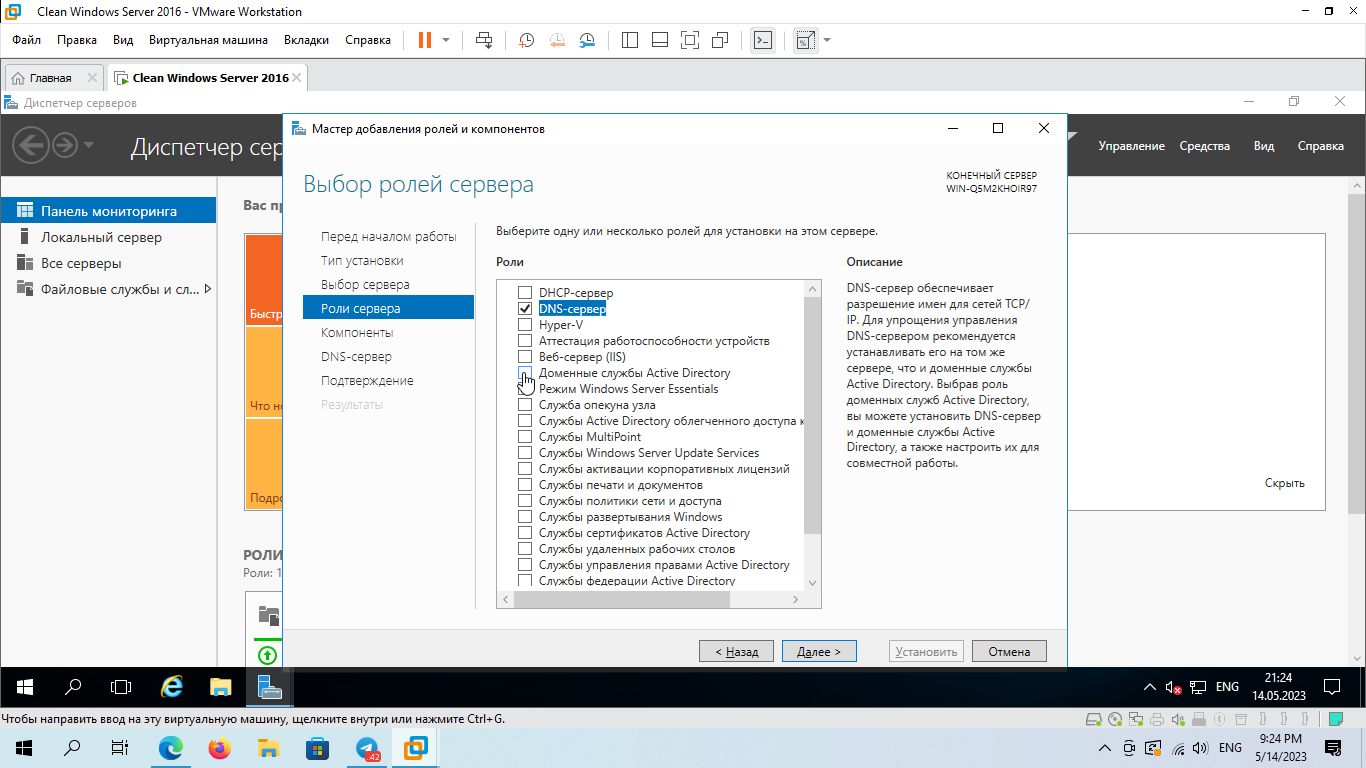
\includegraphics[width=0.85\textwidth]{5_0033}
    \label{img:33}
    \caption{Добавляем роль домееных служб Active Directory}
  \end{figure}

  \begin{figure}[H]
    \centering
    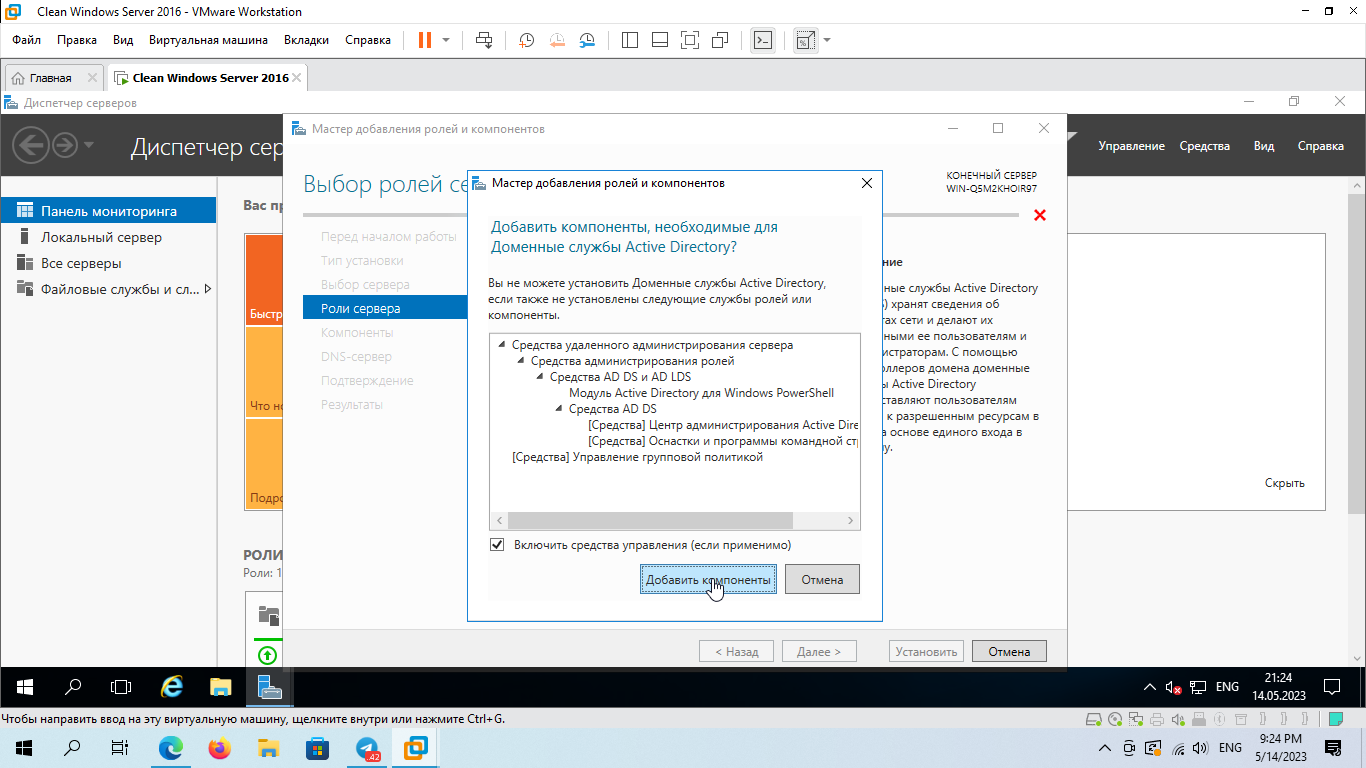
\includegraphics[width=0.85\textwidth]{5_0034}
    \label{img:34}
    \caption{И необходимые компоненты}
  \end{figure}

  \begin{figure}[H]
    \centering
    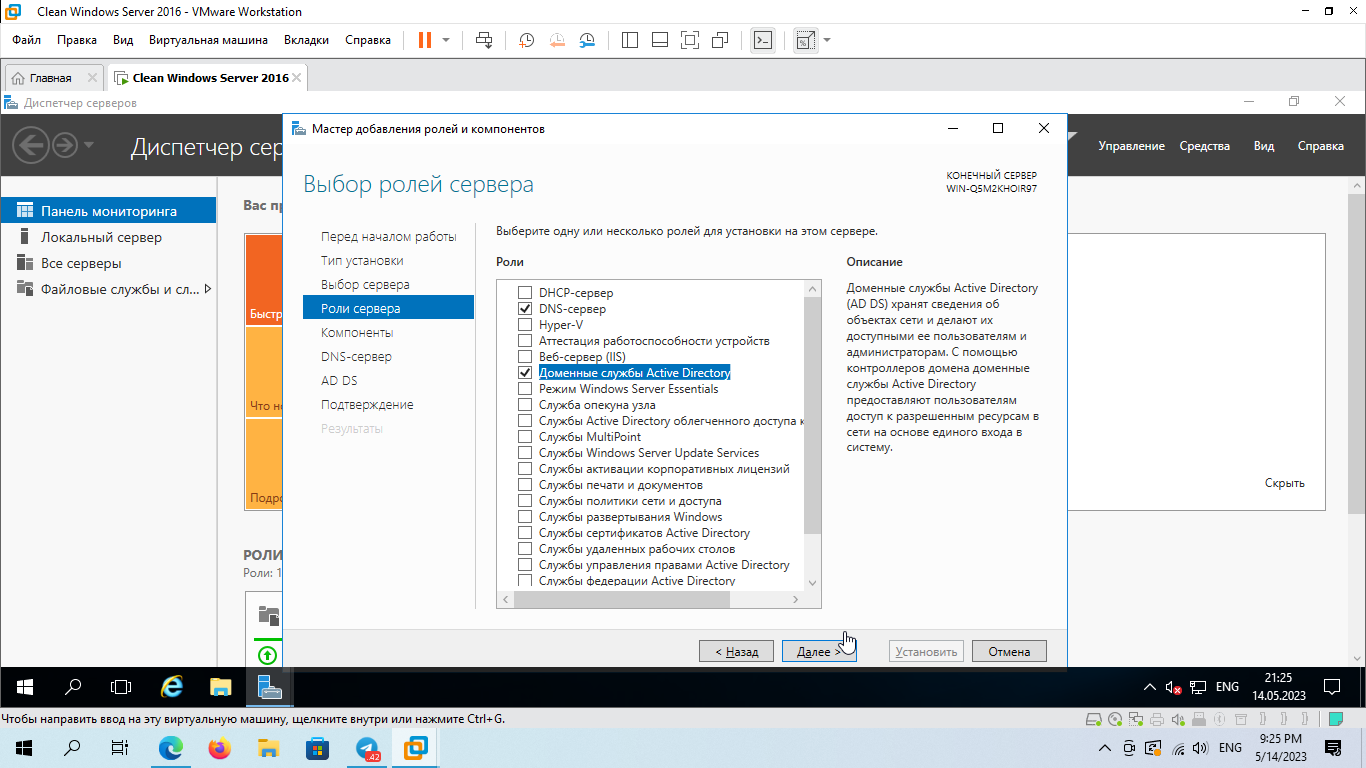
\includegraphics[width=0.85\textwidth]{5_0035}
    \label{img:35}
    \caption{Роли добавлены}
  \end{figure}

  \begin{figure}[H]
    \centering
    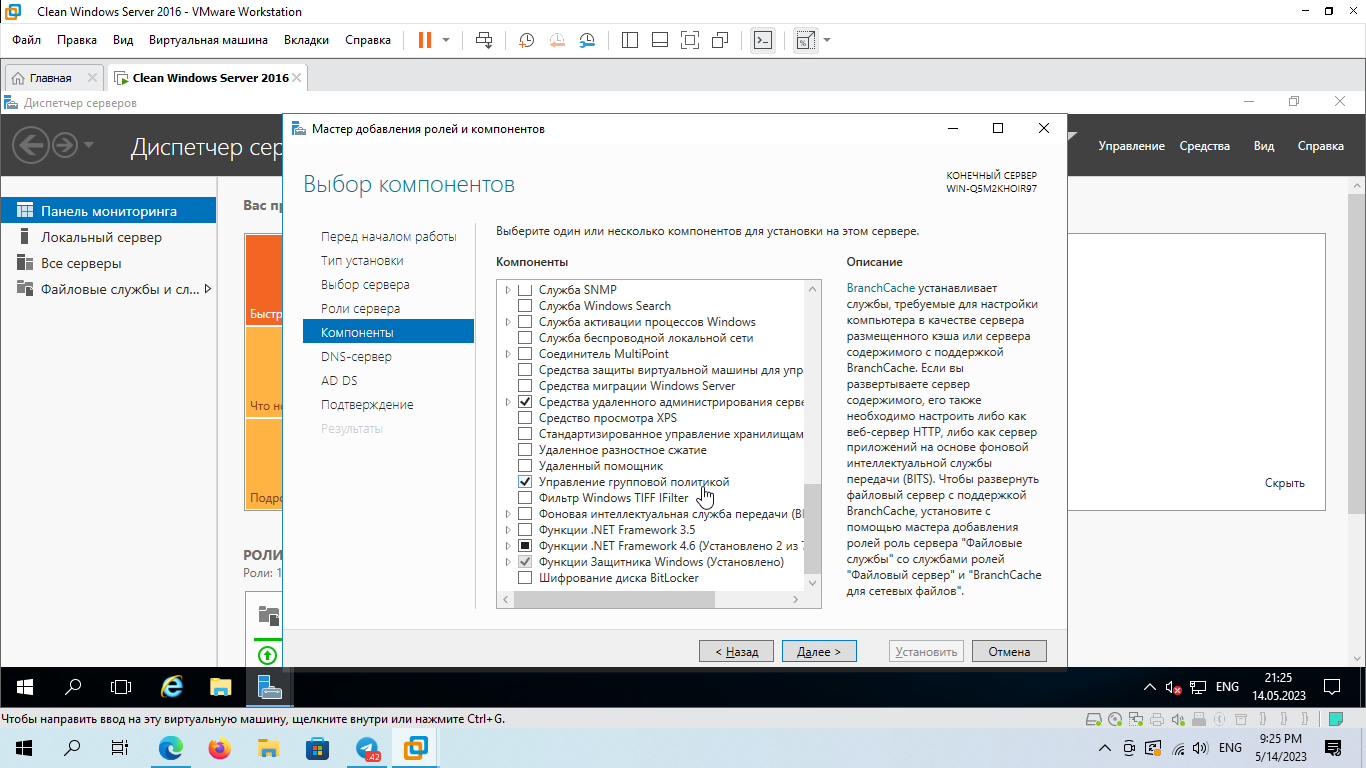
\includegraphics[width=0.85\textwidth]{5_0036}
    \label{img:36}
    \caption{Необходима роль управления груповой политикой}
  \end{figure}

  \begin{figure}[H]
    \centering
    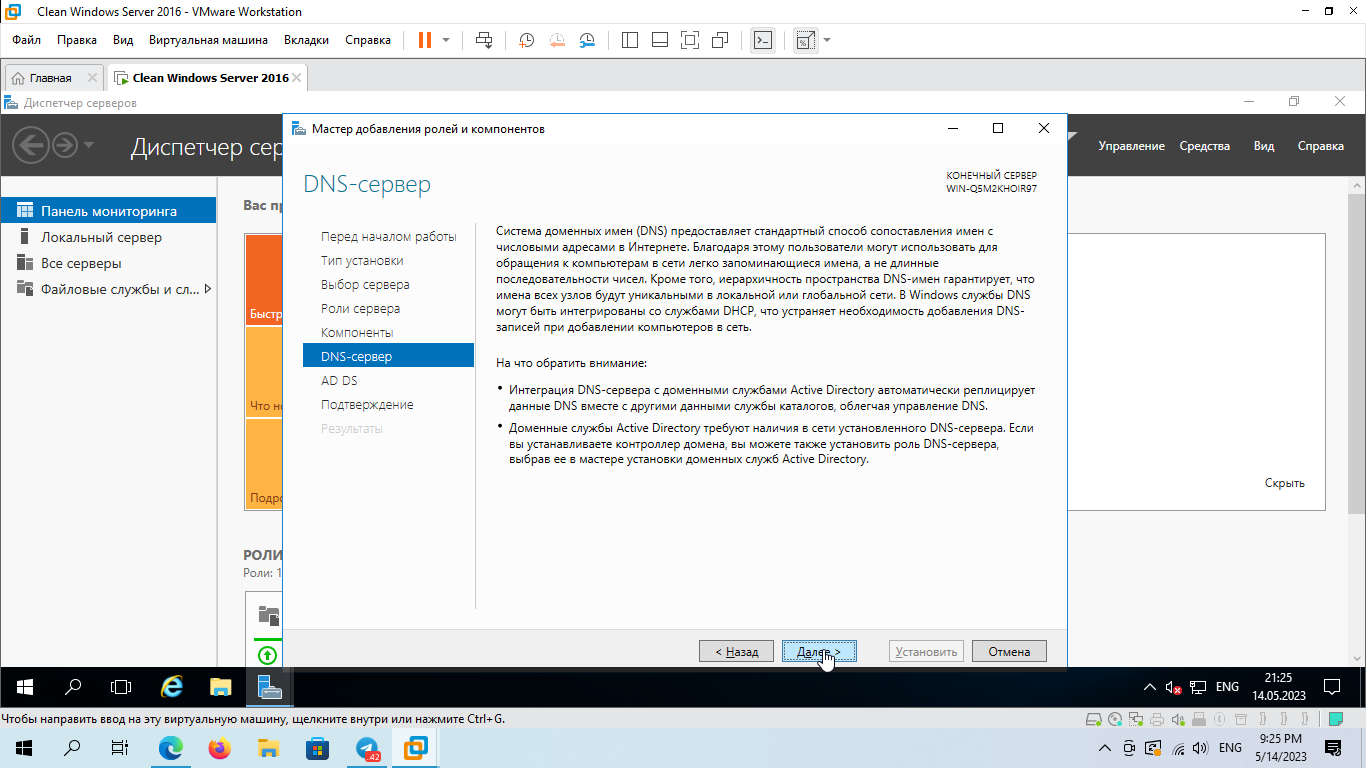
\includegraphics[width=0.85\textwidth]{5_0037}
    \label{img:37}
    \caption{Со всем соглашаемся}
  \end{figure}

  \begin{figure}[H]
    \centering
    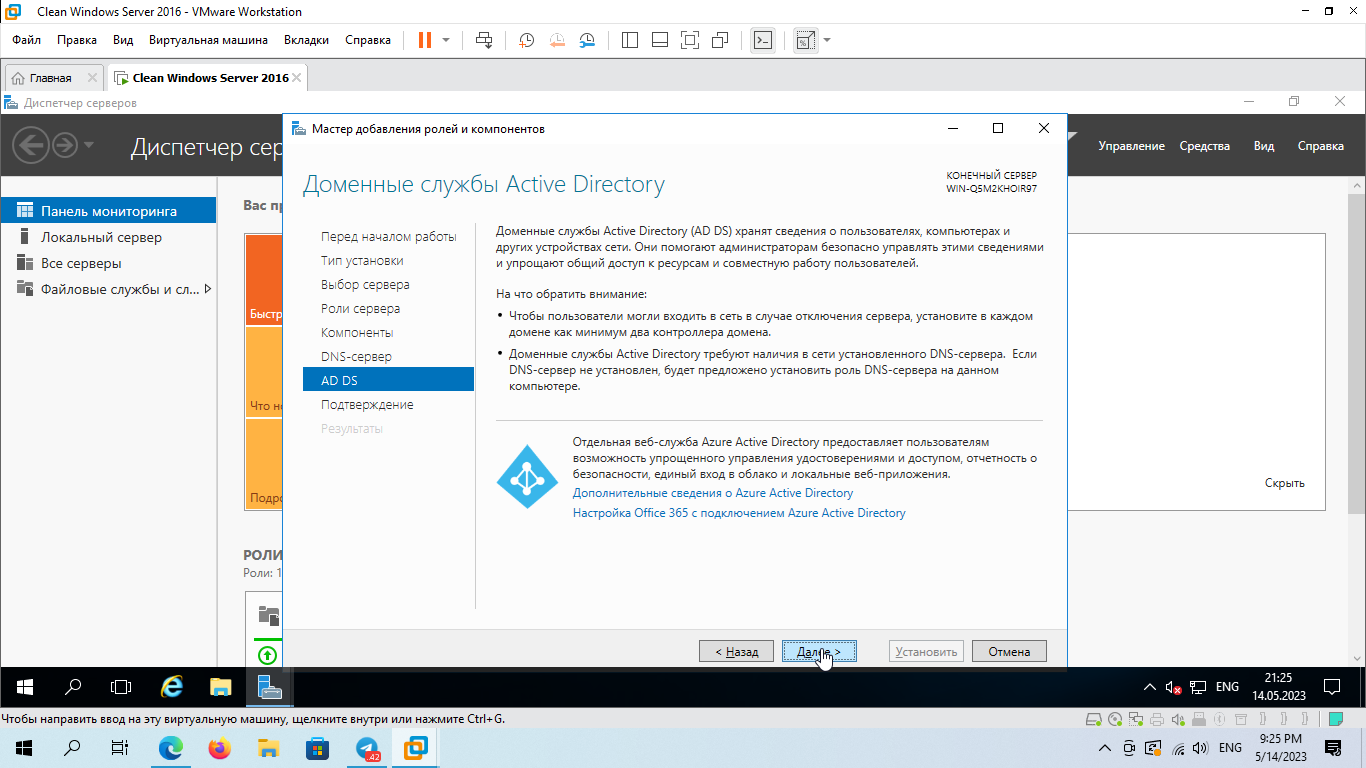
\includegraphics[width=0.85\textwidth]{5_0038}
    \label{img:38}
    \caption{Далее}
  \end{figure}

  \begin{figure}[H]
    \centering
    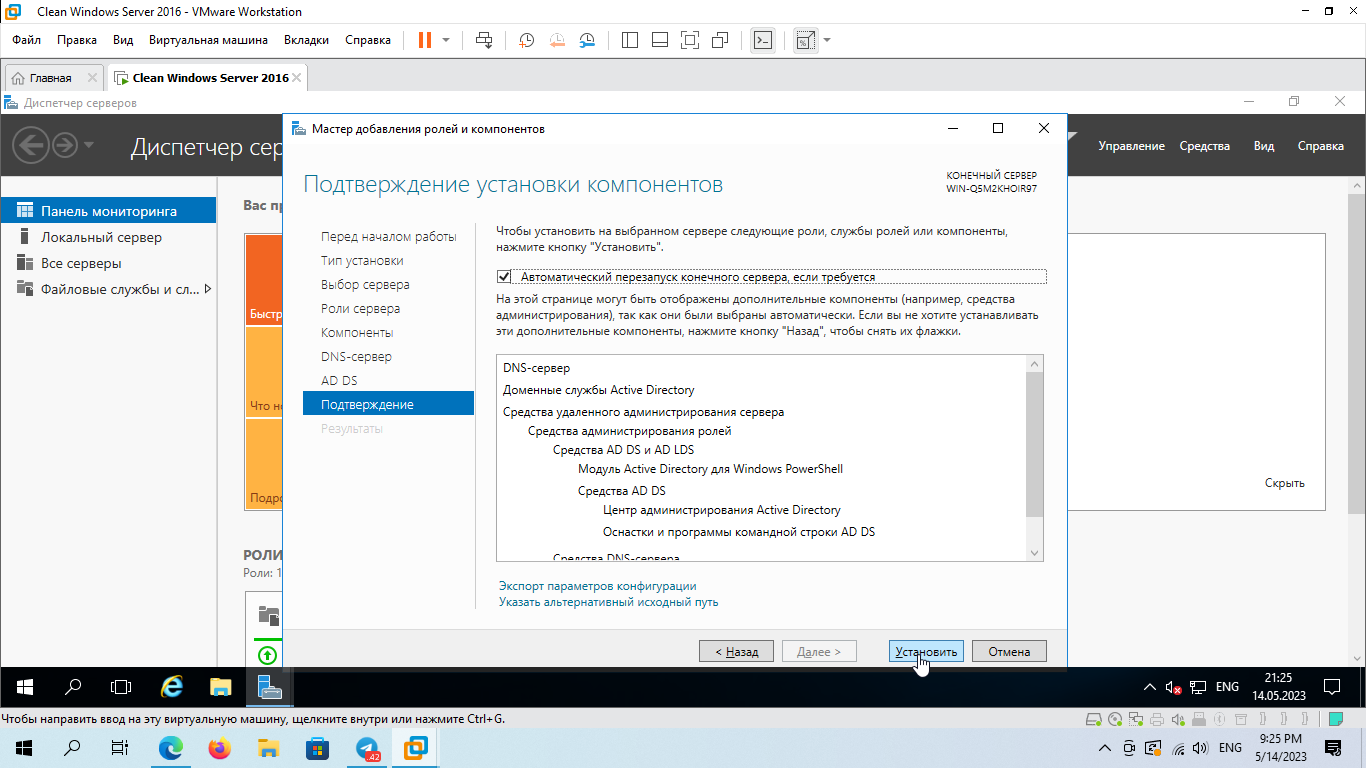
\includegraphics[width=0.85\textwidth]{5_0039}
    \label{img:39}
    \caption{Установить}
  \end{figure}

  \begin{figure}[H]
    \centering
    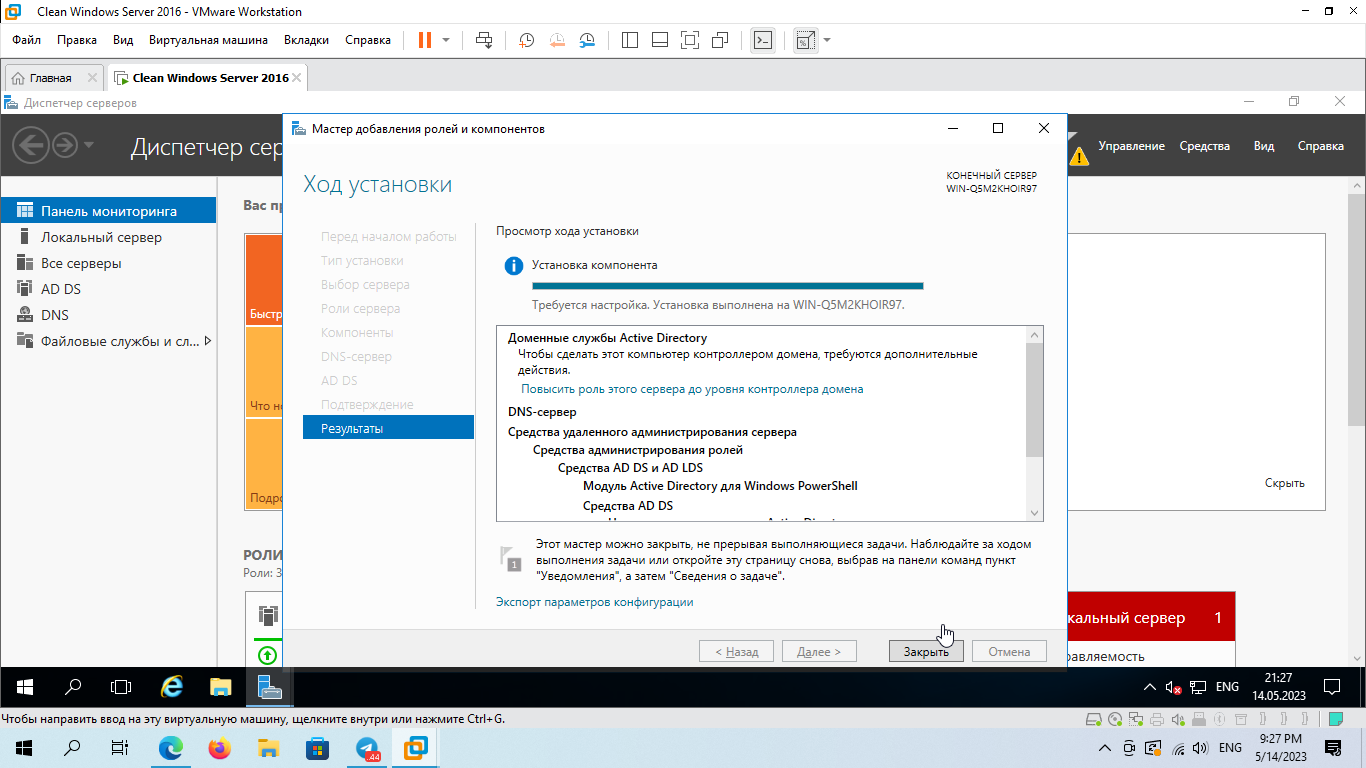
\includegraphics[width=0.85\textwidth]{5_0040}
    \label{img:40}
    \caption{Установка завершена}
  \end{figure}

  \subsubsection{Создание домена}

  \begin{figure}[H]
    \centering
    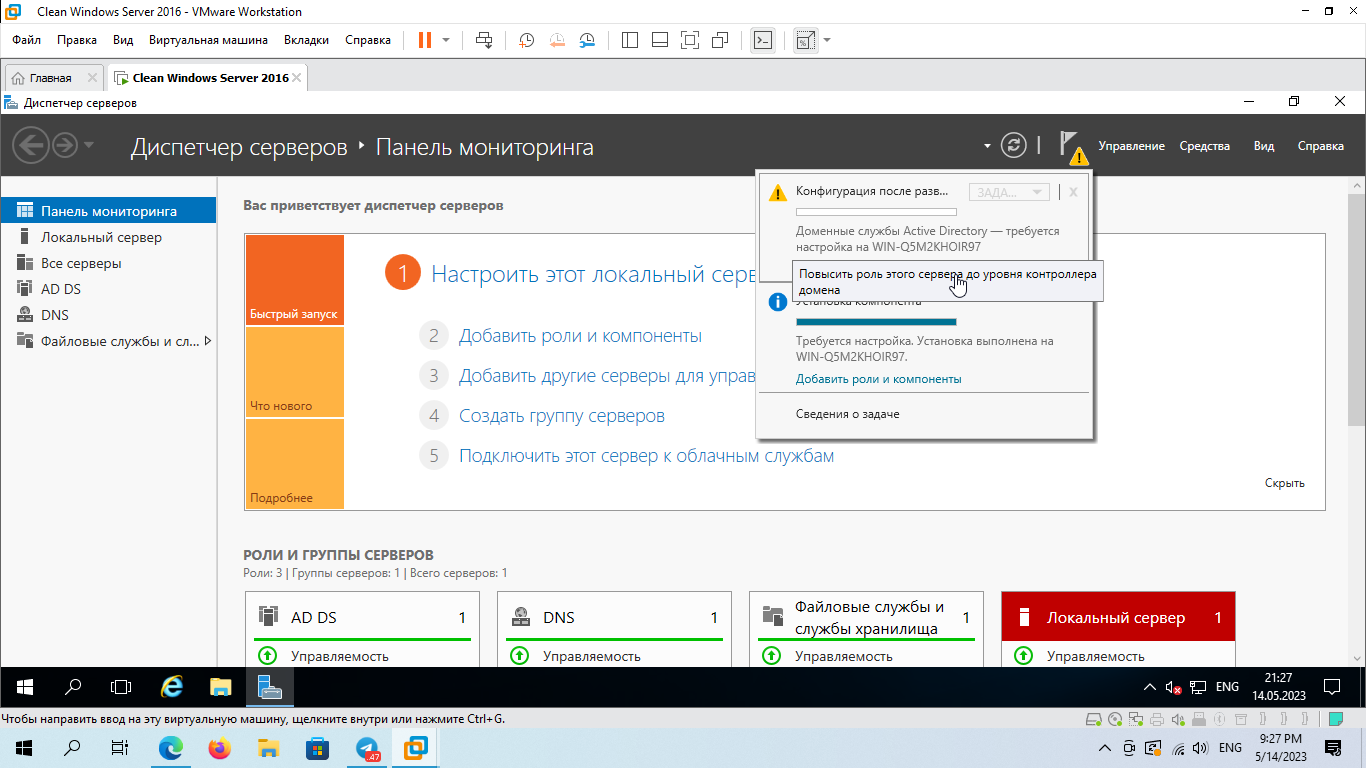
\includegraphics[width=0.85\textwidth]{5_0041}
    \label{img:41}
    \caption{Начинаем повышение роли сервера до контроллера домена}
  \end{figure}

  \begin{figure}[H]
    \centering
    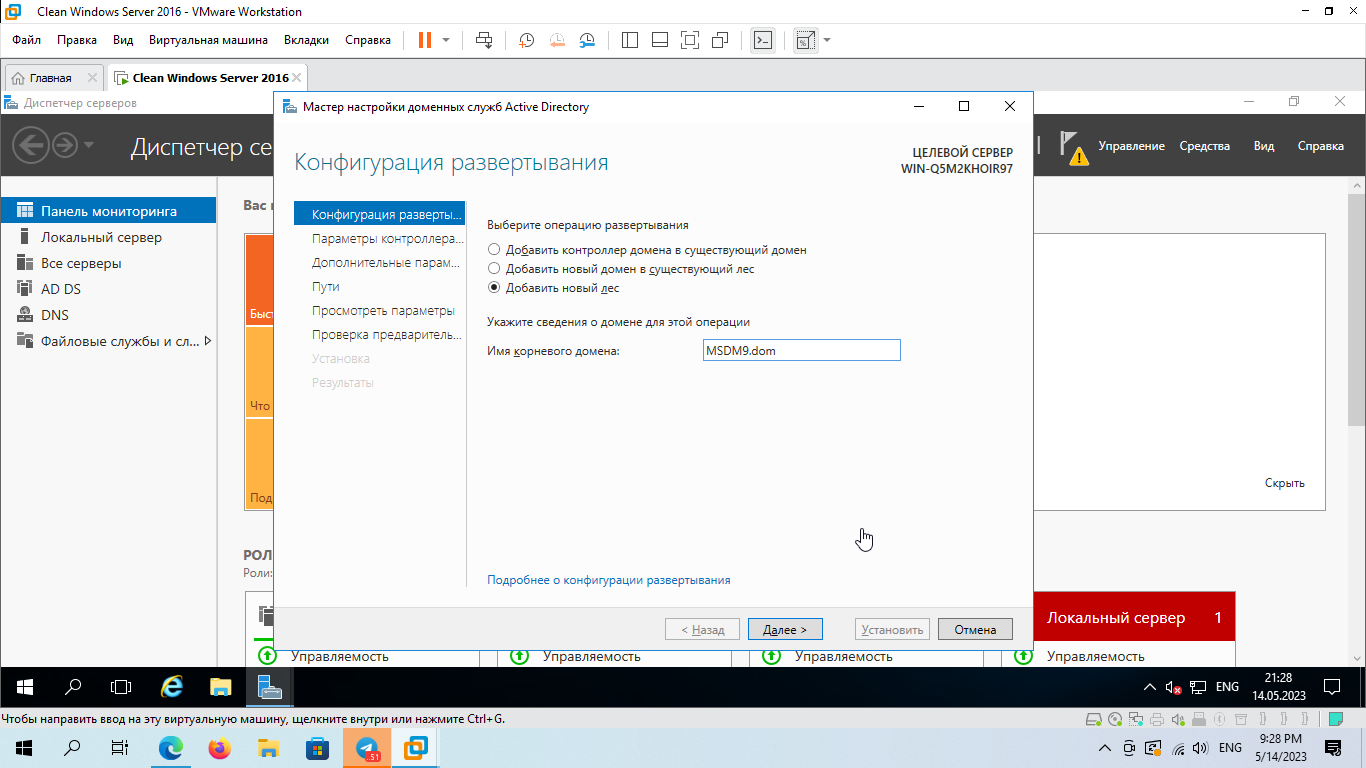
\includegraphics[width=0.85\textwidth]{5_0045}
    \label{img:45}
    \caption{Указываем имя домена}
  \end{figure}

  \begin{figure}[H]
    \centering
    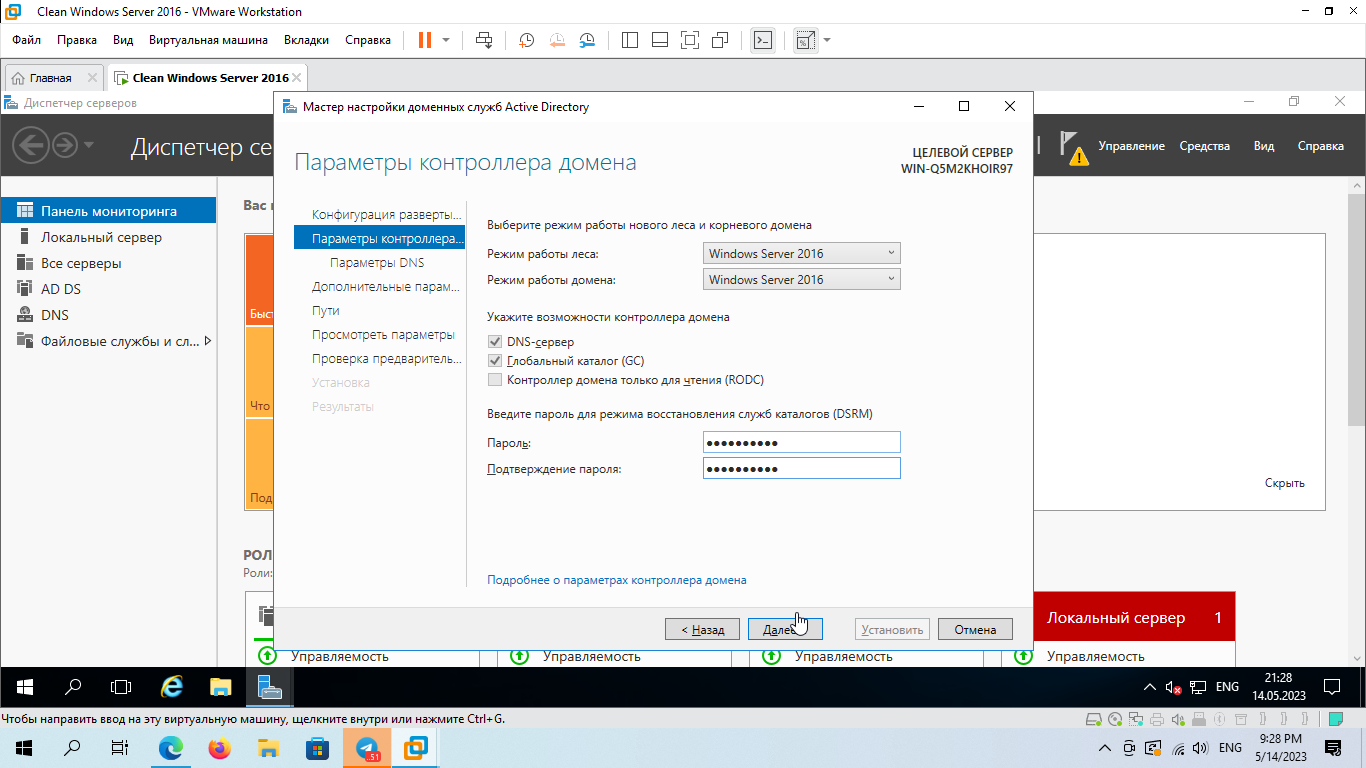
\includegraphics[width=0.85\textwidth]{5_0046}
    \label{img:46}
    \caption{Указываем пароль контроллера домена}
  \end{figure}

  \begin{figure}[H]
    \centering
    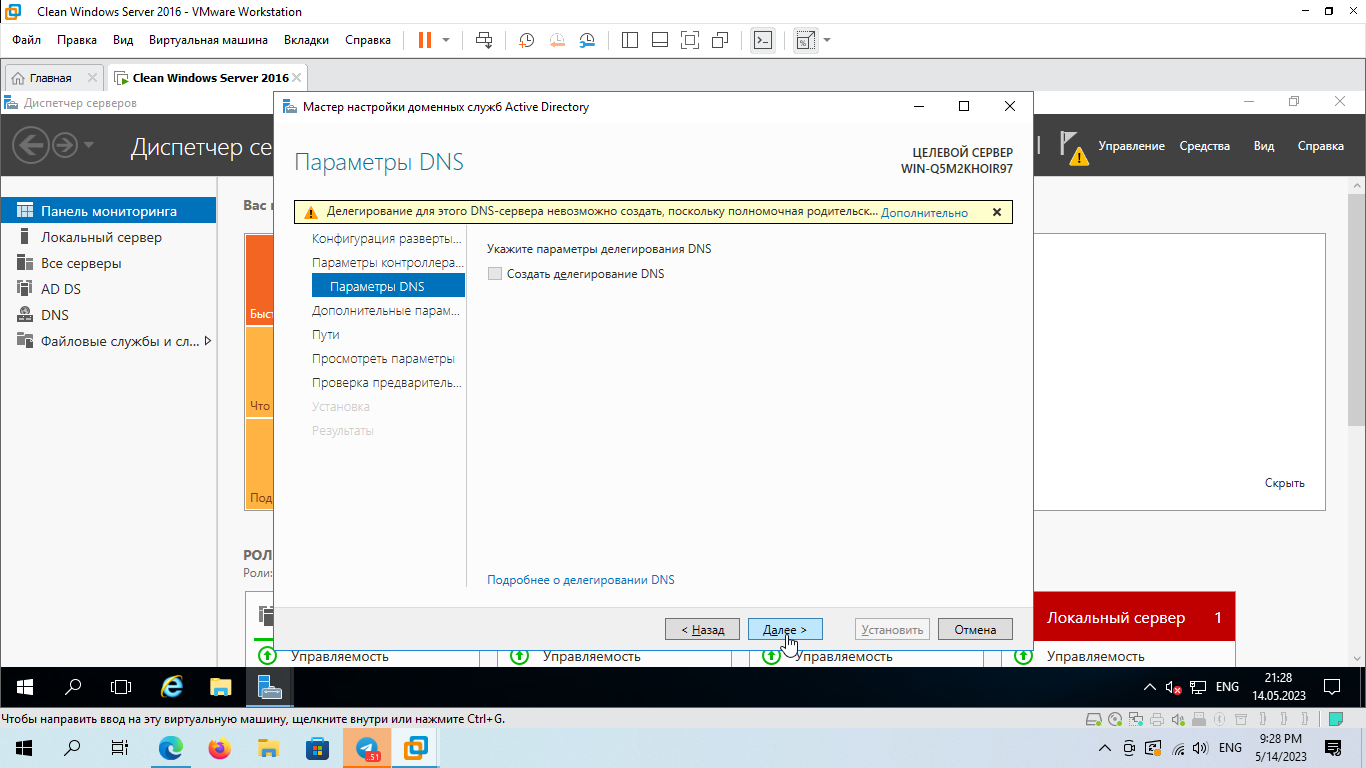
\includegraphics[width=0.85\textwidth]{5_0047}
    \label{img:47}
    \caption{Далее}
  \end{figure}

  \begin{figure}[H]
    \centering
    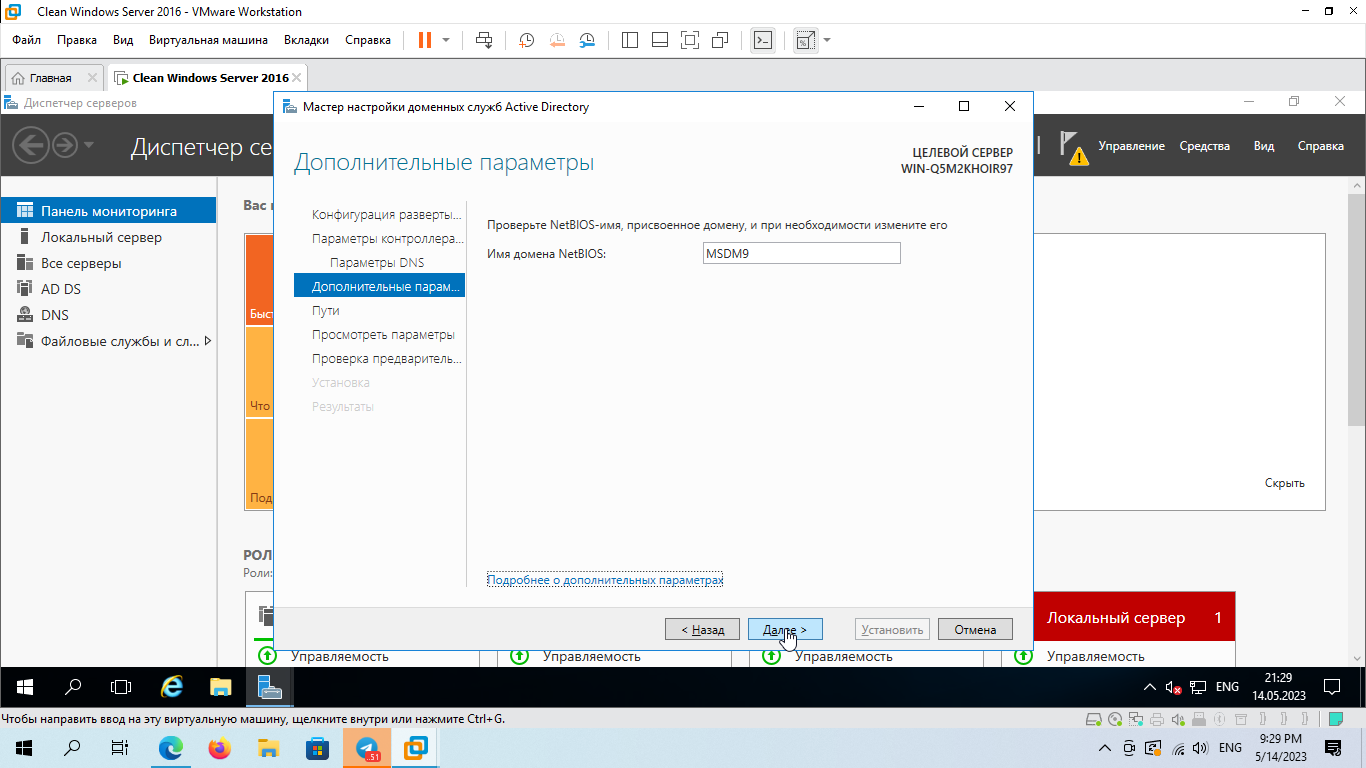
\includegraphics[width=0.85\textwidth]{5_0048}
    \label{img:48}
    \caption{Имя домена NetBIOS установилось автоматически}
  \end{figure}

  \begin{figure}[H]
    \centering
    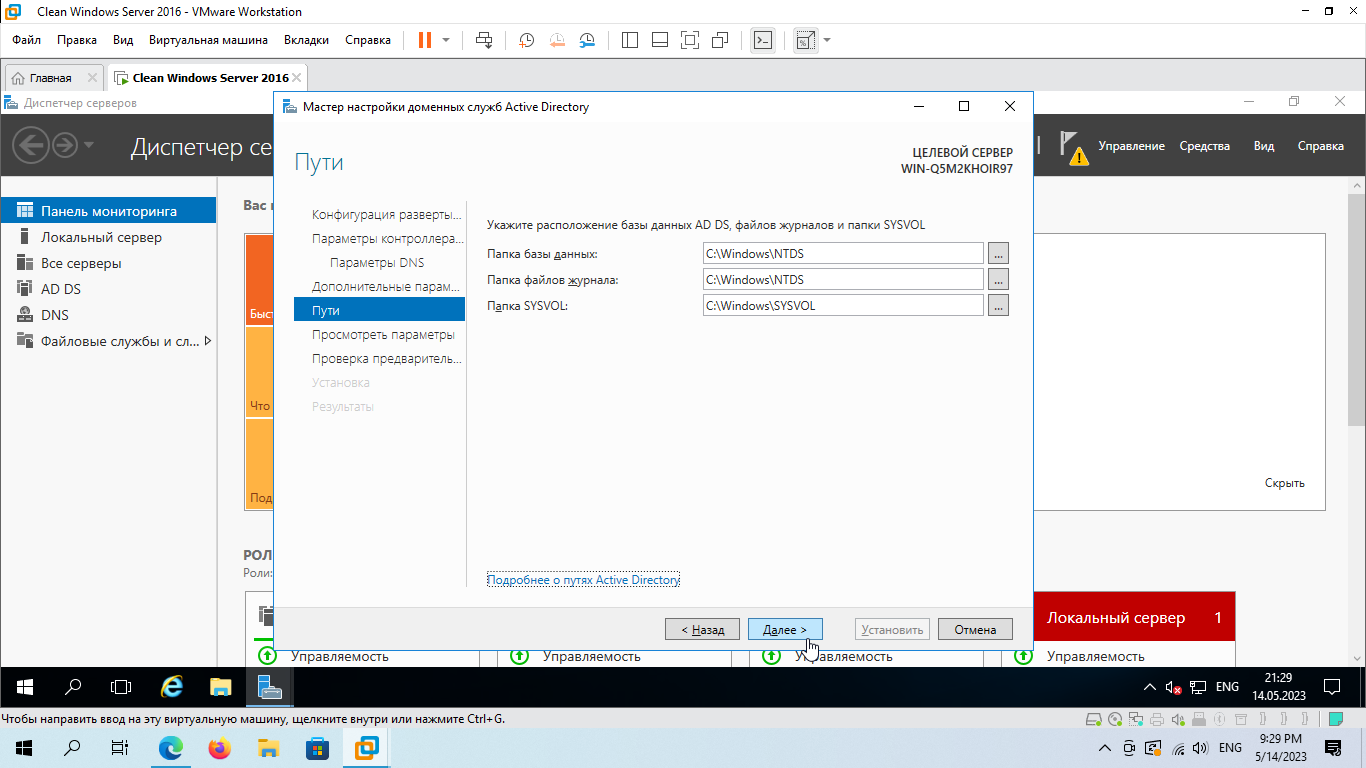
\includegraphics[width=0.85\textwidth]{5_0049}
    \label{img:49}
    \caption{Пути не изменяем}
  \end{figure}

  \begin{figure}[H]
    \centering
    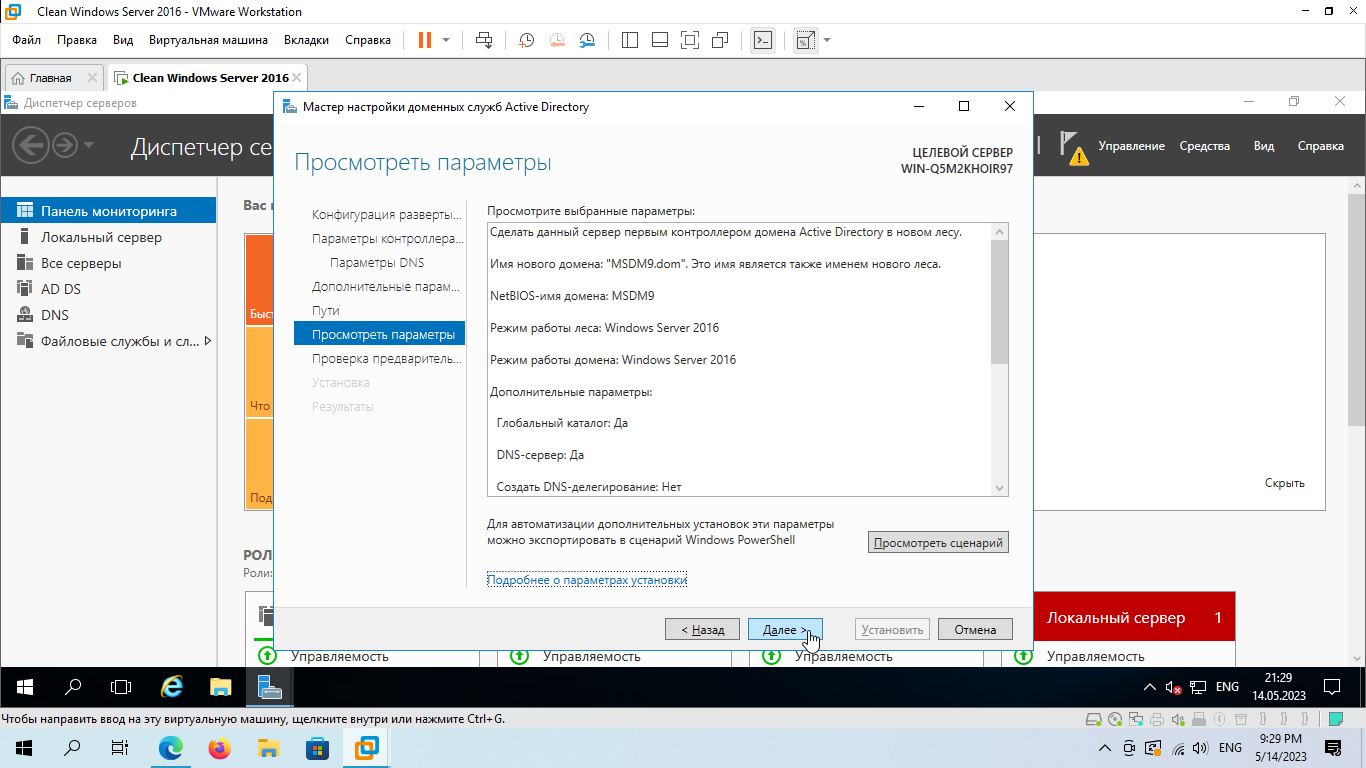
\includegraphics[width=0.85\textwidth]{5_0050}
    \label{img:50}
    \caption{Далее}
  \end{figure}

  \begin{figure}[H]
    \centering
    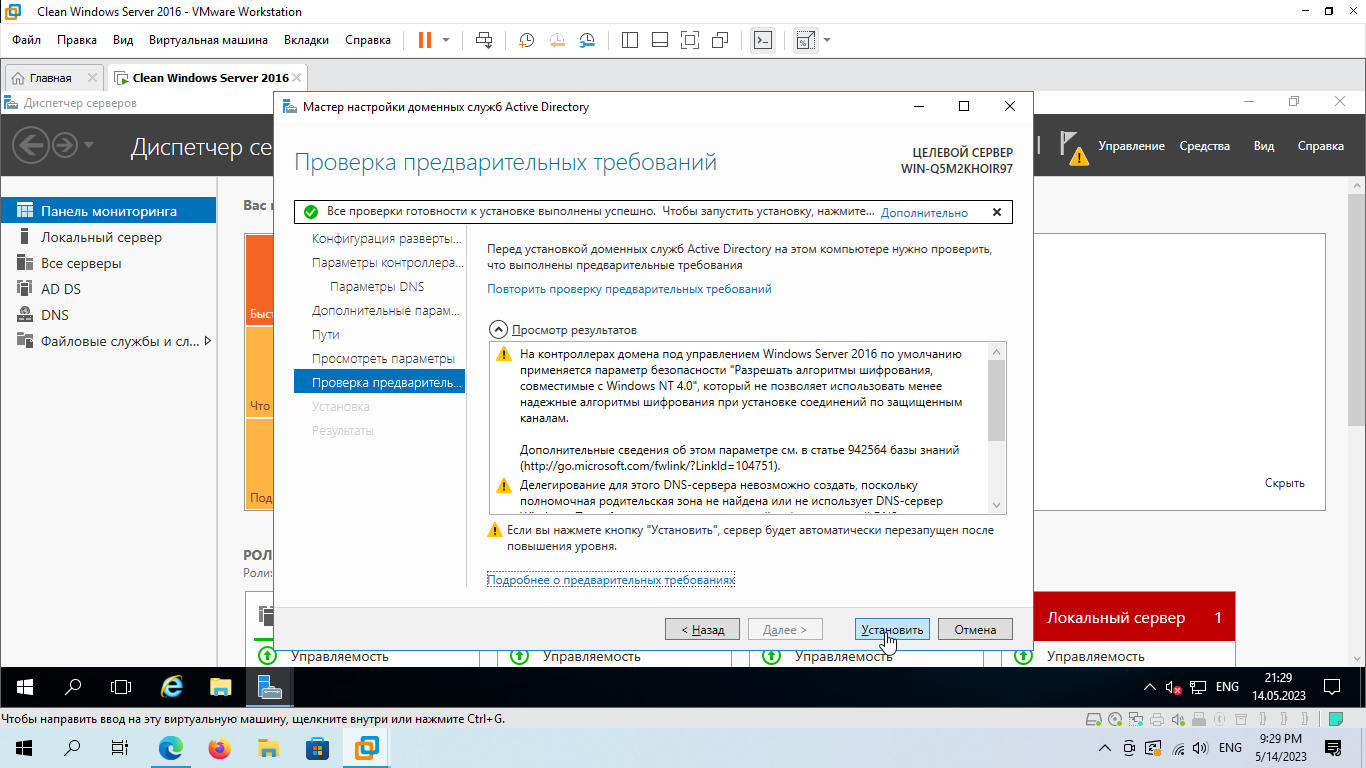
\includegraphics[width=0.85\textwidth]{5_0051}
    \label{img:51}
    \caption{Установить}
  \end{figure}

  \begin{figure}[H]
    \centering
    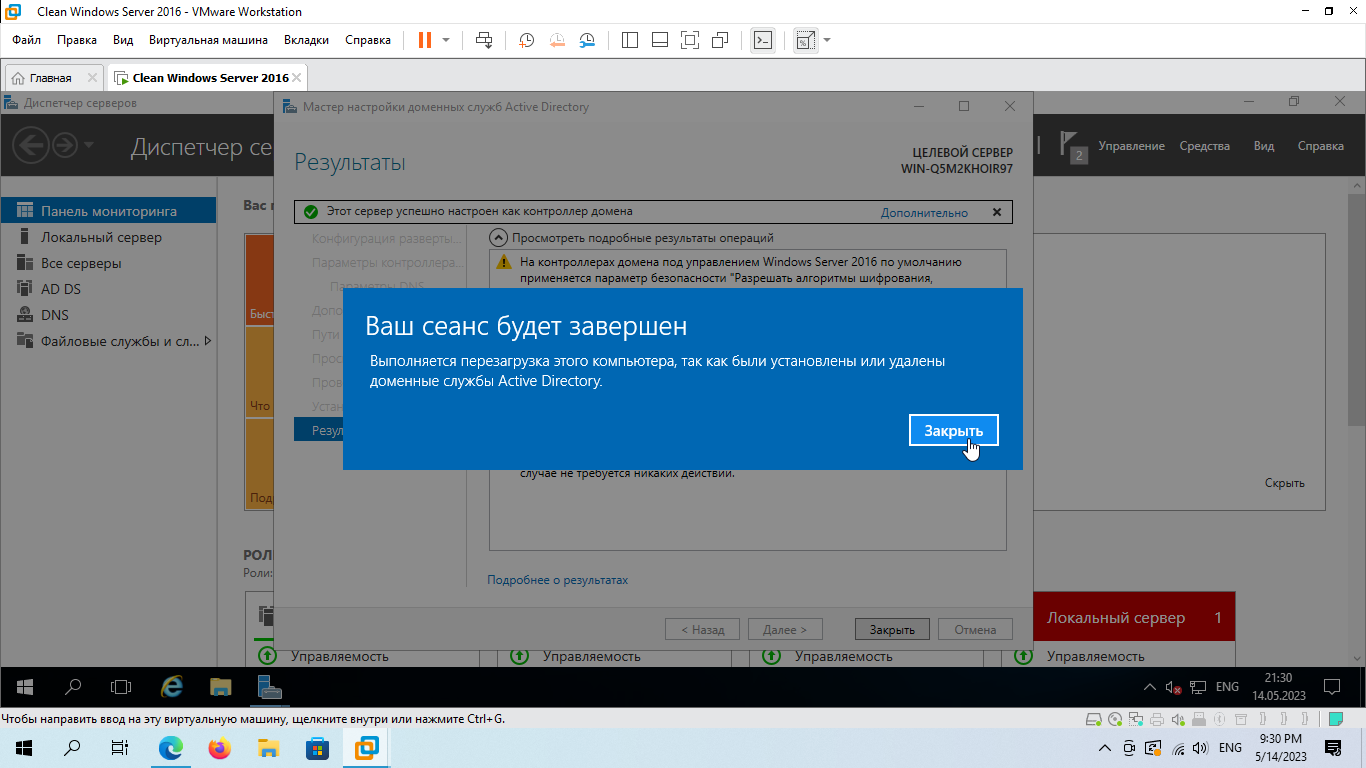
\includegraphics[width=0.85\textwidth]{5_0052}
    \label{img:52}
    \caption{Необходима перезагрузка}
  \end{figure}

  \begin{figure}[H]
    \centering
    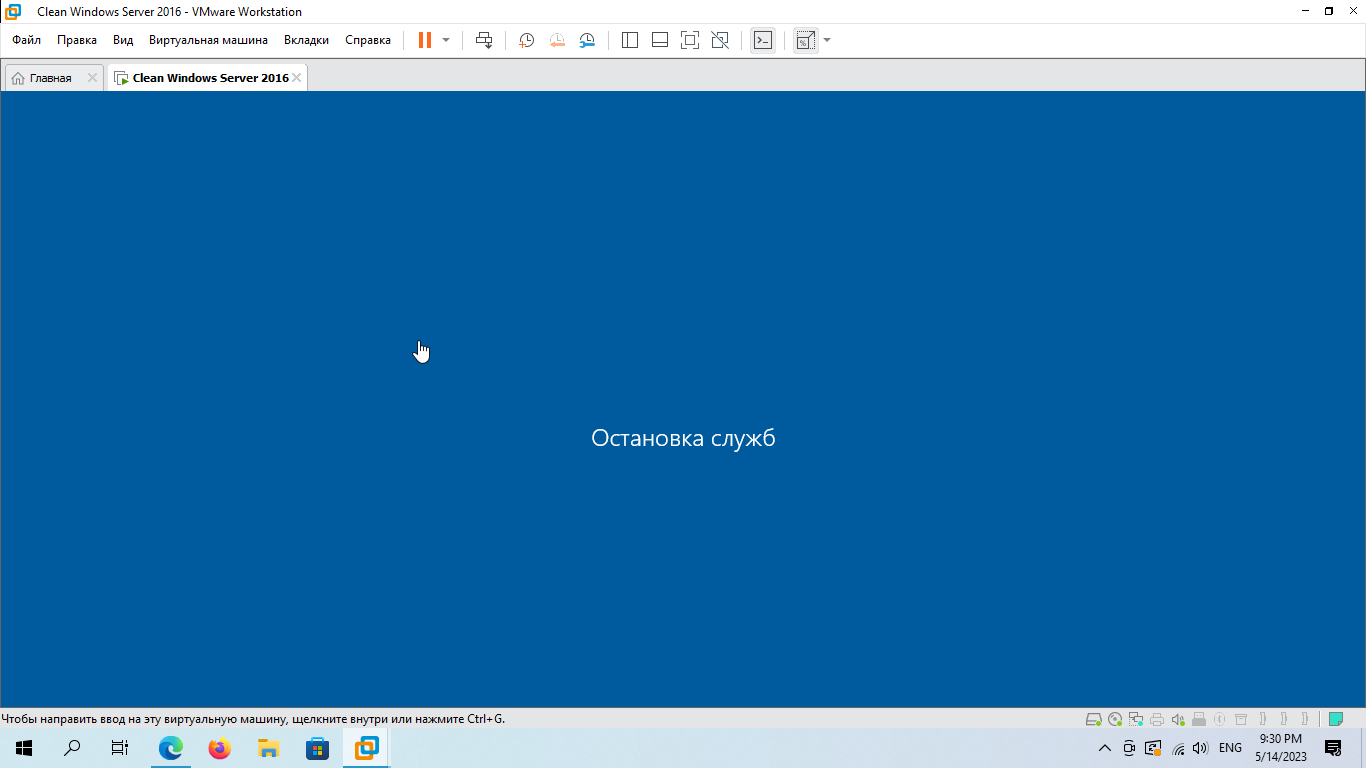
\includegraphics[width=0.85\textwidth]{5_0053}
    \label{img:53}
    \caption{Перезагрузка}
  \end{figure}

  Домен создан и готов к работе.

  \subsection{Настройка клиентской машины}

  Воспользуемся уже готовым образов с Windows 10:

  \begin{figure}[H]
    \centering
    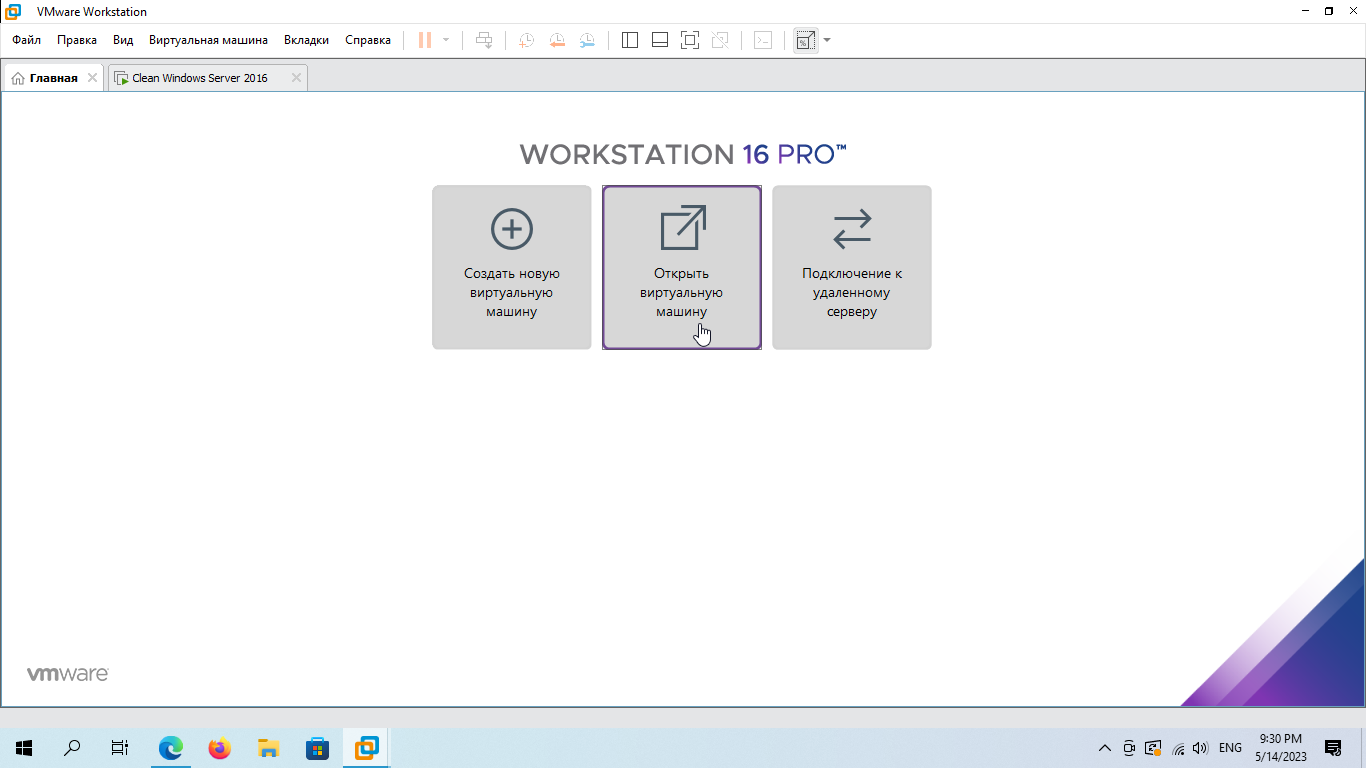
\includegraphics[width=0.85\textwidth]{5_0054}
    \label{img:54}
    \caption{Начинаем импорт ВМ}
  \end{figure}

  \begin{figure}[H]
    \centering
    \includegraphics[width=0.85\textwidth]{5_0055}
    \label{img:55}
    \caption{Указываем путь до образа}
  \end{figure}

  \begin{figure}[H]
    \centering
    \includegraphics[width=0.85\textwidth]{5_0056}
    \label{img:56}
    \caption{Открываем настройки ВМ}
  \end{figure}

  \begin{figure}[H]
    \centering
    \includegraphics[width=0.85\textwidth]{5_0057}
    \label{img:57}
    \caption{Подключаем сетевой адаптер к нужной сети}
  \end{figure}

  \begin{figure}[H]
    \centering
    \includegraphics[width=0.85\textwidth]{5_0058}
    \label{img:58}
    \caption{Загрузка системы}
  \end{figure}

  \begin{figure}[H]
    \centering
    \includegraphics[width=0.85\textwidth]{5_0059}
    \label{img:59}
    \caption{Входим в учетную запись пользователя}
  \end{figure}

  \subsubsection{Настройка сети}

  \begin{figure}[H]
    \centering
    \includegraphics[width=0.85\textwidth]{5_0060}
    \label{img:60}
    \caption{Открываем панель задач}
  \end{figure}

  \begin{figure}[H]
    \centering
    \includegraphics[width=0.85\textwidth]{5_0061}
    \label{img:61}
    \caption{Сеть и Интернет}
  \end{figure}

  \begin{figure}[H]
    \centering
    \includegraphics[width=0.85\textwidth]{5_0062}
    \label{img:62}
    \caption{Центр управления сетями и общим доступом}
  \end{figure}

  \begin{figure}[H]
    \centering
    \includegraphics[width=0.85\textwidth]{5_0064}
    \label{img:64}
    \caption{Выбираем необходимое подключение}
  \end{figure}

  \begin{figure}[H]
    \centering
    \includegraphics[width=0.85\textwidth]{5_0065}
    \label{img:65}
    \caption{Открываем свойства адаптера}
  \end{figure}

  \begin{figure}[H]
    \centering
    \includegraphics[width=0.85\textwidth]{5_0066}
    \label{img:66}
    \caption{Переходим к настройке IPv4}
  \end{figure}

  \begin{figure}[H]
    \centering
    \includegraphics[width=0.85\textwidth]{5_0067}
    \label{img:67}
    \caption{Указываем настройки сети}
  \end{figure}

  В качестве IP адреса машины был выбран первый свободный в данной сети - 192.168.142.3,
  в качестве DNS указан адрес серверной машины - 192.168.142.2.

  \begin{figure}[H]
    \centering
    \includegraphics[width=0.85\textwidth]{5_0068}
    \label{img:68}
    \caption{Проверка доступности}
  \end{figure}

  \begin{figure}[H]
    \centering
    \includegraphics[width=0.85\textwidth]{5_0069}
    \label{img:69}
    \caption{Проверка доступности}
  \end{figure}

  \subsubsection{Начало подключения к домену}

  \begin{figure}[H]
    \centering
    \includegraphics[width=0.85\textwidth]{5_0070}
    \label{img:70}
    \caption{Открываем параметры системы}
  \end{figure}

  \begin{figure}[H]
    \centering
    \includegraphics[width=0.85\textwidth]{5_0071}
    \label{img:71}
    \caption{Пункт "Система"}
  \end{figure}

  \begin{figure}[H]
    \centering
    \includegraphics[width=0.85\textwidth]{5_0072}
    \label{img:72}
    \caption{Дополнительные параметры системы}
  \end{figure}

  \begin{figure}[H]
    \centering
    \includegraphics[width=0.85\textwidth]{5_0073}
    \label{img:73}
    \caption{Вкладка "Имя Компьютера"}
  \end{figure}

  \begin{figure}[H]
    \centering
    \includegraphics[width=0.85\textwidth]{5_0074}
    \label{img:74}
    \caption{Кнопка "Изменить"}
  \end{figure}

  \begin{figure}[H]
    \centering
    \includegraphics[width=0.85\textwidth]{5_0075}
    \label{img:75}
    \caption{Вводим имя компьютера и домен}
  \end{figure}

  \subsection{Создание пользователей на серверной машине}

  Серверная машина перезашрузилась, продолжим работу с ней:

  \begin{figure}[H]
    \centering
    \includegraphics[width=0.85\textwidth]{5_0076}
    \label{img:76}
    \caption{Входим в учетную запись}
  \end{figure}

  \begin{figure}[H]
    \centering
    \includegraphics[width=0.85\textwidth]{5_0077}
    \label{img:77}
    \caption{Переходим к управлению AD DS}
  \end{figure}

  \begin{figure}[H]
    \centering
    \includegraphics[width=0.85\textwidth]{5_0078}
    \label{img:78}
    \caption{переходим к AD DS}
  \end{figure}

  \begin{figure}[H]
    \centering
    \includegraphics[width=0.85\textwidth]{5_0079}
    \label{img:79}
    \caption{Открываем центр администрирования}
  \end{figure}

  \begin{figure}[H]
    \centering
    \includegraphics[width=0.85\textwidth]{5_0080}
    \label{img:80}
    \caption{Центр администрирования открывается}
  \end{figure}

  \begin{figure}[H]
    \centering
    \includegraphics[width=0.85\textwidth]{5_0081}
    \label{img:81}
    \caption{Переходим во вкладку пользователей}
  \end{figure}

  \begin{figure}[H]
    \centering
    \includegraphics[width=0.85\textwidth]{5_0082}
    \label{img:82}
    \caption{Добавляем нового пользователя}
  \end{figure}

  \begin{figure}[H]
    \centering
    \includegraphics[width=0.85\textwidth]{5_0083}
    \label{img:83}
    \caption{Указываем его данные}
  \end{figure}

  \begin{figure}[H]
    \centering
    \includegraphics[width=0.85\textwidth]{5_0084}
    \label{img:84}
    \caption{Добавляем еще одного пользователя}
  \end{figure}

  \begin{figure}[H]
    \centering
    \includegraphics[width=0.85\textwidth]{5_0085}
    \label{img:85}
    \caption{Также указываем его данные}
  \end{figure}

  \begin{figure}[H]
    \centering
    \includegraphics[width=0.85\textwidth]{5_0086}
    \label{img:86}
    \caption{Пользователи добавлены}
  \end{figure}

  \subsection{Подключение к домену и вход в доменную учетную запись}

  \begin{figure}[H]
    \centering
    \includegraphics[width=0.85\textwidth]{5_0087}
    \label{img:87}
    \caption{Подключаемся к домену - ОК}
  \end{figure}

  \begin{figure}[H]
    \centering
    \includegraphics[width=0.85\textwidth]{5_0088}
    \label{img:88}
    \caption{Вводим данные учетной записи Администратора}
  \end{figure}

  \begin{figure}[H]
    \centering
    \includegraphics[width=0.85\textwidth]{5_0089}
    \label{img:89}
    \caption{Подключение к домену прошло успешно}
  \end{figure}

  \begin{figure}[H]
    \centering
    \includegraphics[width=0.85\textwidth]{5_0090}
    \label{img:90}
    \caption{Требуется перезагрузить компьютер}
  \end{figure}

  \begin{figure}[H]
    \centering
    \includegraphics[width=0.85\textwidth]{5_0091}
    \label{img:91}
    \caption{Выполняем перезагрузку}
  \end{figure}

  \begin{figure}[H]
    \centering
    \includegraphics[width=0.85\textwidth]{5_0092}
    \label{img:92}
    \caption{Входим в доменную учетную запись}
  \end{figure}

  \begin{figure}[H]
    \centering
    \includegraphics[width=0.85\textwidth]{5_0093}
    \label{img:93}
    \caption{Необходимо сменить пароль}
  \end{figure}

  \begin{figure}[H]
    \centering
    \includegraphics[width=0.85\textwidth]{5_0094}
    \label{img:94}
    \caption{Указываем новый пароль}
  \end{figure}

  \begin{figure}[H]
    \centering
    \includegraphics[width=0.85\textwidth]{5_0095}
    \label{img:95}
    \caption{Вход}
  \end{figure}

  \begin{figure}[H]
    \centering
    \includegraphics[width=0.85\textwidth]{5_0096}
    \label{img:96}
    \caption{Учетная запись верная}
  \end{figure}

  Проверим, что компьютер отобразился в системе AD DS:

  \begin{figure}[H]
    \centering
    \includegraphics[width=0.85\textwidth]{5_0097}
    \label{img:97}
    \caption{Открываем вкладку с компьютерами}
  \end{figure}

  \begin{figure}[H]
    \centering
    \includegraphics[width=0.85\textwidth]{5_0098}
    \label{img:98}
    \caption{Новый компьютер в списке}
  \end{figure}

  \subsection{Создание нового подразделения}
  \begin{figure}[H]
    \centering
    \includegraphics[width=0.85\textwidth]{5_0099}
    \label{img:99}
    \caption{Открываем "Пользователи и компоненты AD"}
  \end{figure}

  \begin{figure}[H]
    \centering
    \includegraphics[width=0.85\textwidth]{5_0100}
    \label{img:100}
    \caption{Создаем новое подразделение}
  \end{figure}

  \begin{figure}[H]
    \centering
    \includegraphics[width=0.85\textwidth]{5_0101}
    \label{img:101}
    \caption{Указываем имя подразделения}
  \end{figure}

  \begin{figure}[H]
    \centering
    \includegraphics[width=0.85\textwidth]{5_0102}
    \label{img:102}
    \caption{Перемещаем пользователей в подразделение}
  \end{figure}

  \begin{figure}[H]
    \centering
    \includegraphics[width=0.85\textwidth]{5_0103}
    \label{img:103}
    \caption{Указываем необходимое подразделение}
  \end{figure}

  \begin{figure}[H]
    \centering
    \includegraphics[width=0.85\textwidth]{5_0104}
    \label{img:104}
    \caption{Аналогично перемещаем компьютер}
  \end{figure}

  \begin{figure}[H]
    \centering
    \includegraphics[width=0.85\textwidth]{5_0105}
    \label{img:105}
    \caption{В созданное подразделение}
  \end{figure}

  \begin{figure}[H]
    \centering
    \includegraphics[width=0.85\textwidth]{5_0106}
    \label{img:106}
    \caption{Созданное подразделение и его участники}
  \end{figure}

  \subsection{Управление групповой политикой - минимальная длина пароля}

  \begin{figure}[H]
    \centering
    \includegraphics[width=0.85\textwidth]{5_0107}
    \label{img:107}
    \caption{Открываем "Управление групповой политикой"}
  \end{figure}

  \begin{figure}[H]
    \centering
    \includegraphics[width=0.85\textwidth]{5_0108}
    \label{img:108}
    \caption{Открываем нужный лес}
  \end{figure}

  \begin{figure}[H]
    \centering
    \includegraphics[width=0.85\textwidth]{5_0109}
    \label{img:109}
    \caption{Ищем необходимое подразделение}
  \end{figure}

  \begin{figure}[H]
    \centering
    \includegraphics[width=0.85\textwidth]{5_0110}
    \label{img:110}
    \caption{Создаем в нем новый объект групповой политики}
  \end{figure}

  \begin{figure}[H]
    \centering
    \includegraphics[width=0.85\textwidth]{5_0111}
    \label{img:111}
    \caption{указываем имя - gp\_password}
  \end{figure}

  \begin{figure}[H]
    \centering
    \includegraphics[width=0.85\textwidth]{5_0112}
    \label{img:112}
    \caption{Объект политики добавлен}
  \end{figure}

  \begin{figure}[H]
    \centering
    \includegraphics[width=0.85\textwidth]{5_0113}
    \label{img:113}
    \caption{Переходим к его настройкам}
  \end{figure}

  \begin{figure}[H]
    \centering
    \includegraphics[width=0.85\textwidth]{5_0114}
    \label{img:114}
    \caption{Ищем необходимый параметр}
  \end{figure}

  \begin{figure}[H]
    \centering
    \includegraphics[width=0.85\textwidth]{5_0115}
    \label{img:115}
    \caption{В политике учетных записей}
  \end{figure}

  \begin{figure}[H]
    \centering
    \includegraphics[width=0.85\textwidth]{5_0116}
    \label{img:116}
    \caption{Политика паролей}
  \end{figure}

  \begin{figure}[H]
    \centering
    \includegraphics[width=0.85\textwidth]{5_0117}
    \label{img:117}
    \caption{Открываем свойства минимальной длины пароля}
  \end{figure}

  \begin{figure}[H]
    \centering
    \includegraphics[width=0.85\textwidth]{5_0118}
    \label{img:118}
    \caption{Указываем численное значение - 10}
  \end{figure}

  Политика создана, проверим, что она применяется к необходимым учетным записям:

  \begin{figure}[H]
    \centering
    \includegraphics[width=0.85\textwidth]{5_0119}
    \label{img:119}
    \caption{Запускаем "Мастер моделирования групповой политики"}
  \end{figure}

  \begin{figure}[H]
    \centering
    \includegraphics[width=0.85\textwidth]{5_0120}
    \label{img:120}
    \caption{Далее}
  \end{figure}

  \begin{figure}[H]
    \centering
    \includegraphics[width=0.85\textwidth]{5_0121}
    \label{img:121}
    \caption{Работа на текущем контроллере домена}
  \end{figure}

  \begin{figure}[H]
    \centering
    \includegraphics[width=0.85\textwidth]{5_0122}
    \label{img:122}
    \caption{На текущем компьютере}
  \end{figure}

  \begin{figure}[H]
    \centering
    \includegraphics[width=0.85\textwidth]{5_0123}
    \label{img:123}
    \caption{Указываем пользователя и целевой компьютер}
  \end{figure}

  \begin{figure}[H]
    \centering
    \includegraphics[width=0.85\textwidth]{5_0125}
    \label{img:125}
    \caption{Никаких дополнительных параметров эмуляции}
  \end{figure}

  \begin{figure}[H]
    \centering
    \includegraphics[width=0.85\textwidth]{5_0126}
    \label{img:126}
    \caption{Далее}
  \end{figure}

  \begin{figure}[H]
    \centering
    \includegraphics[width=0.85\textwidth]{5_0127}
    \label{img:127}
    \caption{Применяем политику к группам, прошедшим проверку}
  \end{figure}

  \begin{figure}[H]
    \centering
    \includegraphics[width=0.85\textwidth]{5_0128}
    \label{img:128}
    \caption{Применяем политику к компьютерам, прошедшим проверку}
  \end{figure}

  \begin{figure}[H]
    \centering
    \includegraphics[width=0.85\textwidth]{5_0129}
    \label{img:129}
    \caption{Далее}
  \end{figure}

  \begin{figure}[H]
    \centering
    \includegraphics[width=0.85\textwidth]{5_0130}
    \label{img:130}
    \caption{Далее}
  \end{figure}

  \begin{figure}[H]
    \centering
    \includegraphics[width=0.85\textwidth]{5_0131}
    \label{img:131}
    \caption{Далее}
  \end{figure}

  \begin{figure}[H]
    \centering
    \includegraphics[width=0.85\textwidth]{5_0132}
    \label{img:132}
    \caption{Готово}
  \end{figure}

  \begin{figure}[H]
    \centering
    \includegraphics[width=0.85\textwidth]{5_0133}
    \label{img:133}
    \caption{Отчет работы моделирования}
  \end{figure}

  \begin{figure}[H]
    \centering
    \includegraphics[width=0.85\textwidth]{5_0134}
    \label{img:134}
    \caption{Смотрим сведения групповой политики}
  \end{figure}

  Как видно из отчета, необходимая политика действительно применилась к указанной учетной записи - все работает верно.

  \subsection{Управление групповой политикой - скрытие значка Корзины с рабочего стола}

  \begin{figure}[H]
    \centering
    \includegraphics[width=0.85\textwidth]{5_0136}
    \label{img:136}
    \caption{Создаем новый объект групповой политике в подразделении}
  \end{figure}

  \begin{figure}[H]
    \centering
    \includegraphics[width=0.85\textwidth]{5_0137}
    \label{img:137}
    \caption{Указываем имя объекта - gp\_desktop}
  \end{figure}

  \begin{figure}[H]
    \centering
    \includegraphics[width=0.85\textwidth]{5_0138}
    \label{img:138}
    \caption{Переходим к его конфигурированию}
  \end{figure}

  \begin{figure}[H]
    \centering
    \includegraphics[width=0.85\textwidth]{5_0139}
    \label{img:139}
    \caption{Переходим к настройкам рабочего стола}
  \end{figure}

  \begin{figure}[H]
    \centering
    \includegraphics[width=0.85\textwidth]{5_0140}
    \label{img:140}
    \caption{К пункту "Удалить значок <<Корзина>> с рабочего стола"}
  \end{figure}

  \begin{figure}[H]
    \centering
    \includegraphics[width=0.85\textwidth]{5_0141}
    \label{img:141}
    \caption{Включаем данный пункт}
  \end{figure}

  \begin{figure}[H]
    \centering
    \includegraphics[width=0.85\textwidth]{5_0142}
    \label{img:142}
    \caption{Применяем настройки}
  \end{figure}

  \begin{figure}[H]
    \centering
    \includegraphics[width=0.85\textwidth]{5_0143}
    \label{img:143}
    \caption{Опция действительно включена}
  \end{figure}

  Проверим, что все работает с помощью моделирования:

  \begin{figure}[H]
    \centering
    \includegraphics[width=0.85\textwidth]{5_0144}
    \label{img:144}
    \caption{Повторяем предыдущий запрос}
  \end{figure}

  \begin{figure}[H]
    \centering
    \includegraphics[width=0.85\textwidth]{5_0146}
    \label{img:146}
    \caption{еобходимый объект применен}
  \end{figure}

  Проверим все на реальной машине:

  \begin{figure}[H]
    \centering
    \includegraphics[width=0.85\textwidth]{5_0150}
    \label{img:150}
    \caption{Выполняем перезагрузку клиентской машины}
  \end{figure}

  \begin{figure}[H]
    \centering
    \includegraphics[width=0.85\textwidth]{5_0151}
    \label{img:151}
    \caption{Входим в учетную запись пользователя}
  \end{figure}

  \begin{figure}[H]
    \centering
    \includegraphics[width=0.85\textwidth]{5_0152}
    \label{img:152}
    \caption{Корзина действительно исчезла}
  \end{figure}

  \begin{figure}[H]
    \centering
    \includegraphics[width=0.85\textwidth]{5_0153}
    \label{img:153}
    \caption{Исчезла}
  \end{figure}

  \subsection{Создание группы безопасности}

  Создадим новую группу и сделаем так, чтобы "Корзина" пропала только у тех
  пользователей, которые сосотоят в этой группе:

  \begin{figure}[H]
    \centering
    \includegraphics[width=0.85\textwidth]{5_0154}
    \label{img:154}
    \caption{Создадим новую группу}
  \end{figure}

  \begin{figure}[H]
    \centering
    \includegraphics[width=0.85\textwidth]{5_0156}
    \label{img:156}
    \caption{Указываем ее имя}
  \end{figure}

  \begin{figure}[H]
    \centering
    \includegraphics[width=0.85\textwidth]{5_0157}
    \label{img:157}
    \caption{Добавим в нее новых участников}
  \end{figure}

  \begin{figure}[H]
    \centering
    \includegraphics[width=0.85\textwidth]{5_0158}
    \label{img:158}
    \caption{Пользователя winuser\_9\_1}
  \end{figure}

  \begin{figure}[H]
    \centering
    \includegraphics[width=0.85\textwidth]{5_0159}
    \label{img:159}
    \caption{Участники группы}
  \end{figure}

  \begin{figure}[H]
    \centering
    \includegraphics[width=0.85\textwidth]{5_0160}
    \label{img:160}
    \caption{Переходим к настройкам необходимого правила}
  \end{figure}

  \begin{figure}[H]
    \centering
    \includegraphics[width=0.85\textwidth]{5_0161}
    \label{img:161}
    \caption{Необхомо изменить фильтры безопасности}
  \end{figure}

  \begin{figure}[H]
    \centering
    \includegraphics[width=0.85\textwidth]{5_0162}
    \label{img:162}
    \caption{Удаляем ненужный}
  \end{figure}

  \begin{figure}[H]
    \centering
    \includegraphics[width=0.85\textwidth]{5_0163}
    \label{img:163}
    \caption{Да}
  \end{figure}

  \begin{figure}[H]
    \centering
    \includegraphics[width=0.85\textwidth]{5_0164}
    \label{img:164}
    \caption{Начинаем добавление нового фильтра}
  \end{figure}

  \begin{figure}[H]
    \centering
    \includegraphics[width=0.85\textwidth]{5_0165}
    \label{img:165}
    \caption{Указываем необходимую группу}
  \end{figure}

  \begin{figure}[H]
    \centering
    \includegraphics[width=0.85\textwidth]{5_0166}
    \label{img:166}
    \caption{Фильтр добавлен}
  \end{figure}

  Проверим, что все работает при помощи моделирование:
  
  \begin{figure}[H]
    \centering
    \includegraphics[width=0.85\textwidth]{5_0170}
    \label{img:170}
    \caption{Повторим запрос для winuser\_9\_1}
  \end{figure}

  \begin{figure}[H]
    \centering
    \includegraphics[width=0.85\textwidth]{5_0171}
    \label{img:171}
    \caption{Нужная политика применилась}
  \end{figure}

  \begin{figure}[H]
    \centering
    \includegraphics[width=0.85\textwidth]{5_0172}
    \label{img:172}
    \caption{Повторим запрос для winuser\_9\_2}
  \end{figure}

  \begin{figure}[H]
    \centering
    \includegraphics[width=0.85\textwidth]{5_0173}
    \label{img:173}
    \caption{Укажем необходимого пользователя}
  \end{figure}

  \begin{figure}[H]
    \centering
    \includegraphics[width=0.85\textwidth]{5_0174}
    \label{img:174}
    \caption{Политика отклонена - все верно}
  \end{figure}

  Проверим на реальной (виртуальной) машине:

  \begin{figure}[H]
    \centering
    \includegraphics[width=0.85\textwidth]{5_0176}
    \label{img:176}
    \caption{Входим в учетную запись winuser\_9\_2}
  \end{figure}

  \begin{figure}[H]
    \centering
    \includegraphics[width=0.85\textwidth]{5_0177}
    \label{img:177}
    \caption{Корзина есть}
  \end{figure}

  \begin{figure}[H]
    \centering
    \includegraphics[width=0.85\textwidth]{5_0178}
    \label{img:178}
    \caption{Входим в учетную запись winuser\_9\_1}
  \end{figure}

  \begin{figure}[H]
    \centering
    \includegraphics[width=0.85\textwidth]{5_0179}
    \label{img:179}
    \caption{Корзины нет}
  \end{figure}

  Все работает верно.

  \newpage
  \section{Вопросы}

  \begin{enumerate}
    \item {
      \textbf{Опишите, как уже существующий объект групповой политики привязать к нескольким подразделениям?}

      Для этого в необходимом домене нужно "Создать существующий ОГП" в настройках которого
      выбрать определенный объект групповой политики.
    }
    \item {
      \textbf{Как вручную применить политику безопасности, но только для компьютера?}

      Необходимо связать ее с соответствующим объектом службы каталогов. Эту политику
      можно настроить по фильтру безопасности, в котором как раз таки можно
      определить необходимый компьютер.
    }
    \item {
      \textbf{В какой последовательности применяются объекты групповых политик?}

      Применение групповых политик происходит в последовательности, соответствующей иерархии GPO: сначала объект групповой политики сайта, затем домена, затем GPO, связанные с подразделениями в соответствии с их вложенностью.
    }
    \item {
      \textbf{Как узнать к каким версиям операционной системы применим тот или иной параметр групповой политики?}

      Для того, чтобы узнать какие версии поддерживает политика, можно открыть окно ее свойств – там посмотреть на поле Требование к версии или поддерживается. В нем указаны версии ОС, на которых эта политика будет работать.
    }
    \item {
      \textbf{В какие 3 контейнера организованы параметры групповой политики?}

      Windows Settings, Software Settings и Administrative Templates.
    }
    \item {
      \textbf{Как называется базовая групповая политика в чистом созданном домене? }

      Политика домена по умолчанию (Default Domain Policy) и Политика контроллера домена
      по умолчанию (Dofaul Domain Controllers Policy)
    }
  \end{enumerate}

  \newpage
  \section{Вывод}

  В ходе данной работы мной были получена навыки работы с групповыми политиками, их создаение
  и настройкой.

\end{document}
